\documentclass[lang=cn,color=blue,cm,11pt,scheme=chinese,bibend=bibtex,sorting=nty]{elegantbook}

\usepackage{xfrac}
\usepackage{esint}
\usepackage{subfig}
\usepackage{float}
	%\usepackage{aas_macros,amsmath,amssymb,comment,cite,esint,graphicx,mathtools,diagbox}

\usepackage{listings}	
%\usepackage{minted}
\usepackage{tensor}
\usepackage{mathtools}

\newcommand{\jw}[1]{\textcolor[RGB]{65,105,225}{ #1-JW}}
\newcommand{\Mc}[1]{\mathcal{#1}}
\def\a{\alpha}
\def\b{\beta}
\def\c{\chi}
\def\d{\delta}
\def\D{\Delta}
\def\f{\frac}
\def\g{\gamma}
\def\gmn{g _ {\m \n}}
\def\G{\Gamma}
\def\lm{\lambda}
\def\l{\left}
\def\L{\Lambda}
\def\m{\mu} 
\def\n{\nu} 
\def\nn{\nonumber}
\def\pl{\partial}
\def\p{\phi} 
\def\td{\tilde} 
\def\r{\right}
\def\s{\sigma}
\def\S{\Sigma}
\def\t{\theta}
\def\Th{\Theta}
\def\k{\kappa}
\def\ep{\epsilon}
\def\la{\lambda }
\newcommand{\isco}{\text{ISCO}}
\newcommand{\ab}[1]{\left|#1\right|}
\newcommand{\br}[1]{\left[#1\right]}
\newcommand{\cu}[1]{\left\{#1\right\}}
\newcommand{\pa}[1]{\left(#1\right)}
	


\def\bea{\begin{eqnarray}}
\def\eea{\end{eqnarray}}
\def\nn{\nonumber}
	

\newcommand{\ee}{\mathrm{e}} 
\newcommand{\df}{\mathrm{d}}   %积分的微分符号
\newcommand{\dif}{\mathrm{d}}   %微分符号
\newcommand{\qpar}{\quad\par}   
\newcommand{\deri}[3]{\dfrac{\mathrm{d}^{#1}#2}{\mathrm{d}#3^{#1}}}%莱布尼茨导数记号
\newcommand{\pderi}[3]{\dfrac{\partial^{#1}#2}{\partial {#3}^{#1}}}
\newcommand{\sit}[3]{\fint_{#1_#2}^{#1_#3}}
\newcommand{\dfint}[2]{\dfrac{\mathrm{d}#1}{#2}}

\newcommand{\blue}[1]{\textcolor[RGB]{0,0,255}{ #1}}



\title{磁重联简介}
%\subtitle{Elegant\LaTeX{} 经典之作}

\author{}% \& Liam Huang \& syvshc \& sikouhjw \& Osbert Wang}
\institute{}
\date{\today}
%\date{August, 16, 2024}
\version{1.0}
%\bioinfo{自定义}{信息}

\setcounter{tocdepth}{3}

\logo{logo-blue.png}
\cover{cover.png}

% 本文档命令
\usepackage{array}
\newcommand{\ccr}[1]{\makecell{{\color{#1}\rule{1cm}{1cm}}}}

% 修改标题页的橙色带
\definecolor{customcolor}{RGB}{115,45,2}
\colorlet{coverlinecolor}{customcolor}
\usepackage{cprotect}

\addbibresource[location=local]{reference.bib} % 参考文献，不要删除

\begin{document}
	
	\maketitle
	\frontmatter
	\chapter*{前言}
	不同于我们所处的地球环境，宇宙中超过99\%的可见物质都并非固、液、气态，而是处于由带电粒子构成的第四种物质形态：等离子体（Plasma）。从恒星的炽热核心到广袤的星系际介质，从太阳风到黑洞周围的吸积盘，等离子体是构成宇宙高能天体的基本单元。因此，理解等离子体的行为，是揭开宇宙剧烈现象之谜的根本前提。
	
	1942年，Alfvén开创性地提出，可以采用磁流体力学（Magnetohydrodynamics, MHD）来研究宇宙中的等离子体。MHD理论的精髓在于，它将描述电磁场的麦克斯韦方程组与描述流体运动的纳维-斯托克斯方程相结合。这一理论的适用性基于一个关键的宏观近似：在远大于粒子运动微观尺度（如德拜长度）和远低于等离子体振荡频率的条件下，我们可以将复杂的带电粒子系统简化为一个保持电中性、具有良好导电性的单一导电流体。
	
	在MHD框架下，当等离子体被视为理想导体时（在大尺度上，高能天体中的等离子体处于高温、低密度状态，电阻率可以忽略），我们得到一个核心推论：磁冻结定理。该定理指出，磁力线将如同“冻结”在流体中，随其一同运动，这意味着磁场的拓扑结构是永恒不变的。然而，从太阳耀斑到活动星系核的喷流，我们观测到大量储存在磁场中的能量在极短时间内爆发式地被释放出来。如果磁场拓扑无法改变，这种快速的能量释放将无从谈起。
	
	为了解决这一矛盾，磁重联（Magnetic Reconnection）的概念应运而生，是打破磁冻结、改变磁场拓扑、释放磁能的关键物理过程。磁重联的最初灵感源于对太阳耀斑的长期观测，而其核心结构电流片（Current Sheet），则是在上世纪70年代通过人造卫星对地球磁尾的原位探测中被首次直接证实。卫星观测到方向相反的磁场被压缩在极薄的区域内，形成了强度极高的电流，为磁重联理论提供了决定性的观测支持。
	
	磁重联的发生，本质上依赖于局域的耗散机制对磁冻结的破坏。我们可以通过磁感应方程式来理解这一点：
	\begin{equation}
		\frac{\partial \vec{B}}{\partial t} = \vec{\nabla} \times (\vec{v} \times
		\vec{B}) - \vec{\nabla} \times (\eta \vec{\nabla} \times \vec{B})
	\end{equation}
	方程右侧第一项是对流项，代表磁冻结效应；第二项是扩散项，代表由电阻率$\eta$引起的磁场耗散。在宇宙绝大部分空间，$\eta$极小，磁冻结占主导。然而，当方向相反的磁力线被挤压形成薄电流片时，极大的磁场梯度导致电流密度$j$剧增。这会触发局域耗散，使得电流片内部的有效电阻率$\eta$显著增大，从而让扩散项变得不可忽略，最终打破磁冻结。这种“全局理想，局域耗散”的图像，是磁重联的核心。
	
	磁重联模型经历了长足发展：
	
	（1）经典电阻MHD模型：早期的Sweet-Parker模型虽然给出了物理图像，但其重联率太慢。随后的Petschek模型通过引入慢激波结构，实现了更快的重联，标志着理论的重大突破。
	
	（2）无碰撞与动理学模型：MHD的流体描述要求粒子间的碰撞足够频繁（即平均自由程很短）。但在许多天体物理环境中，如稀薄的日冕或黑洞吸积盘，等离子体温度极高、密度极低，导致电子的平均自由程非常长，碰撞效应微乎其微。此时，耗散由霍尔效应、电子惯性等无碰撞的动理学效应主导。这类无碰撞重联的速率非常快，能更好地解释观测。研究这一过程的主要工具是Particle-in-Cell（PIC），它能从第一性原理出发精确描述粒子行为，但其巨大的计算资源消耗是其主要缺点。
	
	当前，磁重联研究的终极前沿，是将其置于爱因斯坦的广义相对论（GR）框架下。在黑洞、中子星等致密天体附近，强大的引力不仅扭曲时空，更引入了参考系拖拽等独特效应。在此背景下，磁重联不再是孤立的电磁过程，而是与时空动力学深度耦合。理解广义相对论磁重联，对于解答银河系中心黑洞（Sgr A*）的X射线耀斑、M87黑洞的相对论性喷流以及伽马射线暴等前沿科学问题至关重要。
	
	\tableofcontents
	
	\mainmatter
	
	\chapter{理论基础}
	
	磁重联，作为宇宙中最基本、最高效的能量转化机制之一，其本质是磁场拓扑的急剧重构。要深入理解这一过程，我们必须首先掌握其发生的物理舞台——等离子体的动力学行为。本章旨在为后续的磁重联模型探讨，构建一个坚实的理论地基。首先，我们将简要回顾广义相对论磁流体动力学（GRMHD）的核心方程，这是在强引力场中描述磁化等离子体的标准语言。随后，为了建立物理直观，我们将回到大家更熟悉的经典MHD框架，快速梳理磁流体静力学、动力学波以及激波等基本概念。
	
	\section{广义相对论性磁流体动力学}
	
	描述磁重联机制的基础便是MHD，而在GR框架下，这一理论被拓展为GRMHD。下面我们先简要介绍一下。
	
	GRMHD的基本方程有：
	
	（1）质量守恒方程：
	\begin{equation}
		\nabla_{\mu} (\rho u^{\mu}) = 0
	\end{equation}
	其中$\rho$是磁流体的静质量密度，$u^{\mu}$是磁流体的4-速，满足归一化条件$u^{\mu} u_{\mu} = - 1$，即独立分量数为3。
	
	（2）能量动量守恒方程：
	\begin{equation}
		\nabla_{\mu} T^{\mu \nu} = 0
	\end{equation}
	磁流体的能动张量$T^{\mu \nu}$可分为流体的能动张量$T^{\mu \nu}_{\text{fluid}}$和电磁场的能动张量$T_{\text{EM}}^{\mu \nu}$：
	\begin{equation}
		T^{\mu \nu} = T^{\mu \nu}_{\text{fluid}} + T_{\text{EM}}^{\mu \nu}
	\end{equation}
	其中，流体的能动张量为：
	\begin{equation}
		T^{\mu \nu}_{\text{fluid}} = h u^{\mu} u^{\nu} + p_g g^{\mu \nu}
	\end{equation}
	$h = \rho + u_g + p_g$为磁流体的焓密度，$p_g$为压强，$u_g$是内能密度。电磁场的能量张量为：
	\begin{equation}
		T_{\text{EM}}^{\mu \nu} = F^{\mu \alpha} F^{\nu}{}_{\alpha} - \frac{1}{4} g^{\mu \nu} F^2
	\end{equation}
	$F^{\mu \nu}$是电磁场张量。
	
	\begin{note}
		在一般情况下，由于高能天体周围是高温、低密度的环境，电阻率几乎为0，此时的等离子体常用理想磁流体来描述。对于理想磁流体，洛伦兹力为0：
		\begin{equation}
			u_{\mu} F^{\mu \nu} = 0
		\end{equation}
		我们可以定义一个磁流体静止系，在该参考系下，电场定义为：
		\begin{equation}
			e^{\nu} \coloneqq u_{\mu} F^{\mu \nu}
		\end{equation}
		也就是说，磁流体自身测得的电场为0。同样地，我们可以定义磁流体静止系下的磁场：
		\begin{equation}
			b^{\nu} \coloneqq u_{\mu} {}^{*}F^{\mu \nu}
		\end{equation}
		其中，${}^{*}F^{\mu \nu} = \frac{1}{2} \epsilon^{\mu \nu \rho \sigma} F_{\rho \sigma}$是电磁场张量的对偶形式。不难发现，$b^{\mu} u_{\mu} = 0$，即独立分量数为3。
		
		上面这个定义的方便之处在于，我们可以利用$b^{\mu}$很轻易地反解出电磁场张量，从而将能量动量方程进行简化，下面我们简单推导一下。
		
		从$b^{\mu}$的定义式出发，我们先消去左边的体元张量。先对两边与$\epsilon_{\mu \alpha \beta \gamma}$进行缩并：
		\begin{align*}
			b^{\mu} \epsilon_{\mu \alpha \beta \gamma} & = \frac{1}{2} \epsilon^{\mu \nu \kappa \lambda} u_{\nu} F_{\lambda \kappa} \epsilon_{\mu \alpha \beta \gamma}\\
			& = - \frac{1}{2} u_{\nu} F_{\lambda \kappa} \delta^{\nu}_{[\alpha} \delta^{\kappa}_{\beta} \delta^{\lambda}_{\gamma]} 3!\\
			& = \frac{1}{2} u_{[\nu} F_{\kappa \lambda]} \delta^{\nu}_{\alpha} \delta^{\kappa}_{\beta} \delta^{\lambda}_{\gamma} 3!\\
			& = \frac{3!}{2} u_{[\alpha} F_{\beta \gamma]}\\
			& = u_{\alpha} F_{\beta \gamma} + u_{\gamma} F_{\alpha \beta} + u_{\beta} F_{\gamma \alpha}
		\end{align*}
		于是：
		\[ b^{\mu} \epsilon_{\mu \alpha \beta \gamma} u^{\alpha} = u^{\alpha} u_{\alpha} F_{\beta \gamma} + u^{\alpha} u_{\gamma} F_{\alpha \beta} + u^{\alpha} u_{\beta} F_{\gamma \alpha} = F_{\gamma \beta} \]
		整理一下可得：
		\[ F^{\mu \nu} = \epsilon^{\mu \nu \kappa \lambda} u_{\kappa} b_{\lambda} \]
		代入电磁场能动张量：
		\begin{align*}
			T_{\text{EM}}^{\mu \nu} & = F^{\mu \alpha} F^{\nu}{}_{\alpha} - \frac{1}{4} g^{\mu \nu} F^2\\
			& = \epsilon^{\mu \alpha \kappa \lambda} u_{\kappa} b_{\lambda} \epsilon^{\nu}{}_{\alpha}{}^{\rho \sigma} u_{\rho} b_{\sigma} - \frac{1}{4} g^{\mu \nu} (- 1) 2! 2! \delta^{\kappa}_{[\alpha} \delta^{\lambda}_{\beta]} u_{\kappa} b_{\lambda} u^{\alpha} b^{\beta}\\
			& = g^{\nu \tau} \epsilon^{\mu \alpha \kappa \lambda} u_{\kappa} b_{\lambda} \epsilon_{\tau \alpha \rho \sigma} u^{\rho} b^{\sigma} + \frac{1}{2} g^{\mu \nu} (u_{\alpha} b_{\beta} u^{\alpha} b^{\beta} - u_{\beta} b_{\alpha} u^{\alpha} b^{\beta})\\
			& = - g^{\nu \tau} 3! \delta^{\mu}_{[\tau} \delta^{\kappa}_{\rho} \delta^{\lambda}_{\sigma]} u_{\kappa} b_{\lambda} u^{\rho} b^{\sigma} - \frac{1}{2} g^{\mu \nu} b^2\\
			& = - 3! \delta^{\mu}_{\tau} \delta^{\kappa}_{\rho} \delta^{\lambda}_{\sigma} u_{\kappa} b_{\lambda} g^{\nu [\tau} u^{\rho} b^{\sigma]} - \frac{1}{2} g^{\mu \nu} b^2\\
			& = - 3! u_{\kappa} b_{\lambda} g^{\nu [\mu} u^{\kappa} b^{\lambda]} - \frac{1}{2} g^{\mu \nu} b^2\\
			& = - (g^{\nu \mu} u^{\kappa} b^{\lambda} + g^{\nu \kappa} u^{\lambda} b^{\mu} + g^{\nu \lambda} u^{\mu} b^{\kappa} - g^{\nu \mu} u^{\lambda} b^{\kappa} - g^{\nu \kappa} u^{\mu} b^{\lambda} - g^{\nu \lambda} u^{\kappa} b^{\mu}) u_{\kappa} b_{\lambda} - \frac{1}{2} g^{\mu \nu} b^2\\
			& = - (- g^{\nu \mu} b^2 + 0 + 0 - 0 - u^{\nu} u^{\mu} b^2 + g^{\nu \lambda} b^{\mu} b_{\lambda}) - \frac{1}{2} g^{\mu \nu} b^2\\
			& = b^2 u^{\mu} u^{\nu} + \frac{1}{2} g^{\mu \nu} b^2 - b^{\mu} b^{\nu}
		\end{align*}
		于是，磁流体的能动张量可以写成：
		\begin{equation}
			T^{\mu \nu} = (h + b^2) u^{\mu} u^{\nu} + (p_g + p_b) g^{\mu \nu} - b^{\mu} b^{\nu}
		\end{equation}
		其中，$p_b \equiv \frac{1}{2} b^2$称为磁压。注意，第一项的$b^2 = b^{\mu} b_{\mu}$是一个洛伦兹不变量，代表了流体静止系下测得的磁场能量密度。
		
		此外，我们也经常会用$b^{\mu}$表示出${}^{*}F^{\mu \nu}$：
		\begin{align*}
			{}^{*}F^{\mu \nu} & = \frac{1}{2} \epsilon^{\mu \nu \kappa \lambda} \epsilon_{\kappa \lambda \alpha \beta} u^{\alpha} b^{\beta}\\
			& = - \frac{1}{2} 2! 2! \delta^{\mu}_{[\alpha} \delta^{\nu}_{\beta]} u^{\alpha} b^{\beta}\\
			& = - (u^{\mu} b^{\nu} - u^{\nu} b^{\mu})\\
			& = b^{\mu} u^{\nu} - b^{\nu} u^{\mu}
		\end{align*}
	\end{note}
	
	\begin{note}
		在磁重联模型计算中，我们常常结合有源麦克斯韦方程，将上述能量动量守恒方程进行简化，下面我们简单推导一下。
		
		将磁流体能动张量代入可得：
		\begin{equation}
			\nabla_{\mu} (h u^{\mu} u^{\nu}) = - \nabla^{\nu} p_g - \nabla_{\mu} T^{\mu \nu}_{\text{EM}}
		\end{equation}
		其中：
		\begin{align*}
			\nabla_{\mu} T^{\mu \nu}_{\text{EM}} & = (\nabla_{\mu} F^{\mu \alpha}) F^{\nu}{}_{\alpha} + F^{\mu \alpha} \nabla_{\mu} F^{\nu}{}_{\alpha} - \frac{1}{4} \nabla^{\nu} (F^{\rho \sigma} F_{\rho \sigma})\\
			& = - J^{\alpha} F^{\nu}{}_{\alpha} + F_{\mu \alpha} \nabla^{\mu} F^{\nu \alpha} - \frac{1}{2} F_{\mu \alpha} \nabla^{\nu} F^{\mu \alpha}\\
			& = - J^{\alpha} F^{\nu}{}_{\alpha} + \frac{1}{2} F_{\mu \alpha} \nabla^{\mu} F^{\nu \alpha} - \frac{1}{2} F_{\mu \alpha} \nabla^{\alpha} F^{\nu \mu} - \frac{1}{2} F_{\mu \alpha} \nabla^{\nu} F^{\mu \alpha}\\
			& = - J^{\alpha} F^{\nu}{}_{\alpha} + \frac{3}{2} F_{\mu \alpha} \nabla^{[\mu} F^{\nu \alpha]}\\
			& = - J^{\alpha} F^{\nu}{}_{\alpha}
		\end{align*}
		于是最终能量动量守恒方程化为：
		\begin{equation}
			\nabla_{\mu} (h u^{\mu} u^{\nu}) = - \nabla^{\nu} p_g + J^{\alpha} F^{\nu}{}_{\alpha}
		\end{equation}
	\end{note}
	
	（3）麦克斯韦方程：
	\begin{equation}
		\nabla_{\mu} F^{\mu \nu} = - J^{\nu}, \quad \nabla_{\nu} {}^{*}F^{\mu \nu} = 0
	\end{equation}
	其中，$J^{\mu}$为4-电流密度，$\rho_e' = - J_{\nu} u^{\nu}$为流体静止系下测得的电荷密度。
	
	（4）欧姆定律：
	\begin{equation}
		F^{\mu}{}_{\nu} u^{\nu} = \eta (J^{\mu} - \rho_e' u^{\mu})
	\end{equation}
	可以看到，在没有电阻率时，该方程等价于洛伦兹力为0，即对应于理想磁流体。
	
	\begin{note}
		理想磁流体的一个重要的结论就是磁冻结原理，下面我们简单推导一下。
		
		我们先回顾一下麦克斯韦方程组：
		\begin{equation}
			\left\{ \begin{aligned}
				& \vec{\nabla} \cdot \vec{E} = \rho_e\\
				& \vec{\nabla} \times \vec{E} = - \frac{\partial \vec{B}}{\partial t}\\
				& \vec{\nabla} \cdot \vec{B} = 0\\
				& \vec{\nabla} \times \vec{B} = \frac{\partial \vec{E}}{\partial t} + \vec{j}
			\end{aligned} \right.
		\end{equation}
		以及欧姆定律：
		\begin{equation}
			\vec{j} = \sigma (\vec{E} + \vec{v} \times \vec{B})
		\end{equation}
		$\sigma$为电导率。在天体物理领域，电场的位移通常可以忽略，即$\frac{\partial \vec{E}}{\partial t} \approx 0$，于是我们有：
		\begin{equation}
			\vec{\nabla} \times (\eta \vec{\nabla} \times \vec{B}) = \vec{\nabla} \times \vec{E} + \vec{\nabla} \times (\vec{v} \times \vec{B})
		\end{equation}
		整理一下便得到磁感应方程式：
		\begin{equation}
			\frac{\partial \vec{B}}{\partial t} = \vec{\nabla} \times (\vec{v} \times \vec{B}) - \vec{\nabla} \times (\eta \vec{\nabla} \times \vec{B})
		\end{equation}
		对于理想磁流体，方程右边第二项耗散项为0：
		\begin{equation}
			\frac{\partial \vec{B}}{\partial t} = \vec{\nabla} \times (\vec{v} \times \vec{B})
		\end{equation}
		\begin{center}
			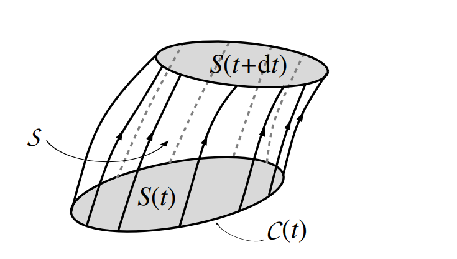
\includegraphics[width=0.5\textwidth]{figures/磁重联简介-1.pdf}
		\end{center}
		
		在$t$时刻，我们考虑一个闭合曲线$C(t)$围成的一个曲面$S(t)$，经过该曲面的磁通量为：
		\begin{equation}
			\Phi (t) = \int_{S (t)} \vec{B} (t) \cdot d \vec{S}
		\end{equation}
		经过$dt$时间后，曲面$S(t)$上的磁流体运动到$S(t+dt)$曲面。这一过程中，磁通量的变化为：
		\begin{equation}
			\frac{d \Phi}{d t} = \lim_{d t \rightarrow 0} \frac{1}{d t} \left[ \int_{S (t + d t)} \vec{B} (t + d t) \cdot d \vec{S} - \int_{S (t)} \vec{B} (t) \cdot d \vec{S} \right]
		\end{equation}
		我们记$dt$时间内曲线$C(t)$扫过的面为$\mathcal{S}$，于是曲面$S(t)$、曲面$S(t+dt)$和曲面$\mathcal{S}$组成一个闭合曲面。在$t+dt$时刻，磁场经过该闭合曲面的磁通量为0：
		\begin{equation}
			\int_{S (t + d t)} \vec{B} (t + d t) \cdot d \vec{S} - \int_{S (t)} \vec{B} (t + d t) \cdot d \vec{S} + \int_{\mathcal{S}} \vec{B} (t + d t) \cdot d \vec{\mathcal{S}} = 0
		\end{equation}
		其中，$d \vec{\mathcal{S}} = d \vec{r} \times \vec{v} dt$，$d\vec{r}$为曲线$C(t)$的线元。于是磁通量的变化量为：
		\begin{equation}
			\begin{aligned}
				\frac{d \Phi}{d t} & = \lim_{d t \rightarrow 0} \frac{1}{dt} \left[ \int_{S (t)} \vec{B} (t + d t) \cdot d \vec{S} - \int_{\mathcal{S}} \vec{B} (t + d t) \cdot d \vec{\mathcal{S}} - \int_{S (t)} \vec{B} (t) \cdot d \vec{S} \right] \\
				& = \int_{S (t)} \frac{\partial \vec{B}}{\partial t} \cdot d \vec{S} - \int_{C (t)} \vec{B} \cdot (d \vec{r} \times \vec{v})\\
				& = \int_{S (t)} \frac{\partial \vec{B}}{\partial t} \cdot d \vec{S} - \int_{C (t)} (\vec{v} \times \vec{B}) \cdot d \vec{r}\\
				& = \int_{S (t)} \left( \frac{\partial \vec{B}}{\partial t} - \vec{\nabla} \times (\vec{v} \times \vec{B}) \right) \cdot d \vec{S}\\
				& = 0
			\end{aligned}
		\end{equation}
		也就是说，对于任意闭合曲面，随着其中磁流体的运动，磁力线的数量并不会减少，磁力线如同被冻结在磁流体中，随之运动。
		
		除了磁通量守恒以外，下面定义的磁螺度也是守恒的：
		\begin{equation}
			H = \int_V (\vec{A} \cdot \vec{B}) d V
		\end{equation}
		其中，$\vec{A}$为磁矢势，$\vec{A} \cdot \vec{B}$称为磁螺度密度。磁螺度是表征磁螺管内部的扭绕和不同磁螺管之间耦合或交连程度的物理量，在一定程度上反映了磁场的拓扑结构。由此可见，理想磁流体的磁力线拓扑结构不变。磁螺度的守恒比磁通量守恒更严格，它约束了磁场的整体拓扑扭缠结构。磁重联正是通过在局部打破理想条件，使得磁螺度可以在小尺度上耗散，从而允许大尺度磁场拓扑发生改变。
	\end{note}
	
	\begin{note}
		除了上面这些方程，有时我们还会用到物态方程。一般来说，我们考虑磁流体是绝热、不可压缩的。绝热过程给出：
		\begin{equation}
			p_g V^{\hat{\gamma}} = \text{const}
		\end{equation}
		其中，$\hat{\gamma}$为绝热指数，一般取值为$4/3 \sim 5/3$，其中$4/3$对应相对性磁流体情形。结合热力学第一定律：
		\begin{equation}
			d (u_g V) = - p_g d V
		\end{equation}
		能得到内能与压强的关系：
		\begin{equation}
			p_g = (\hat{\gamma} - 1) u_g
		\end{equation}
		在计算温度时，我们常用理想气体物态方程：
		\begin{equation}
			p_g = \frac{\rho}{m_p} k_B T_p
		\end{equation}
		其中，$m_p$表示离子质量（一般取氢离子），$T_p$为表示离子温度。电子温度一般由以下经验公式给出：
		\begin{equation}
			\frac{T_p}{T_e} = R_h \frac{\beta^2}{1 + \beta^2} + R_l \frac{1}{1 + \beta^2}
		\end{equation}
		其中$\beta = p_g / p_b$为气压与磁压比值，$R_l$和$R_h$为参数。
	\end{note}
	
	\section{时空3+1分解}
	
	前面我们介绍了GRMHD基本方程的协变形式，接下来便是讨论如何求解这些方程。一个最直接的方法便是在一个具体的坐标系直接计算。不过，这也会带来一个明显的缺陷，以BL坐标系下的Kerr时空为例，坐标$t$在能层内为类空坐标而非类时坐标，导致能层内的物理意义不够明晰。天文领域更偏好对时空进行3+1分解，进而演化3维子空间中的物理量。3+1分解的方式不唯一，但一般指的是下面这种ZAMO系的分解方式。虽然下面这种分解方式指标有些混乱，与一般的3+1分解写法略有不同，表达式稍显复杂，不过由于是针对Kerr时空，实际计算时很多项都会消失。下面我们简单介绍一下。
	
	\subsection{Kerr时空}
	
	我们先回顾一下BL坐标系$\{ t, r, \theta, \phi \}$下的Kerr度规及其逆：（几何单位制下$G = M = c = 1$）
	\begin{equation}
		g_{\mu \nu} = \begin{pmatrix}
			- 1 + \frac{2 r}{\Sigma} & 0 & 0 & - \frac{2 a r \sin^2 \theta}{\Sigma}\\
			0 & \frac{\Sigma}{\Delta} & 0 & 0\\
			0 & 0 & \Sigma & 0\\
			- \frac{2 a r \sin^2 \theta}{\Sigma} & 0 & 0 & \frac{\Xi}{\Sigma} \sin^2 \theta
		\end{pmatrix}
	\end{equation}
	\begin{equation}
		g^{\mu \nu} = \begin{pmatrix}
			- \frac{\Xi}{\Sigma \Delta} & 0 & 0 & - \frac{2 a r}{\Sigma \Delta}\\
			0 & \frac{\Delta}{\Sigma} & 0 & 0\\
			0 & 0 & \frac{1}{\Sigma} & 0\\
			- \frac{2 a r}{\Sigma \Delta} & 0 & 0 & \frac{(\sin^{- 2} \theta - a^2 \Delta^{- 1})}{\Sigma}
		\end{pmatrix}
	\end{equation}
	其中：
	\begin{equation}
		\Sigma = r^2 + a^2 \cos^2 \theta, \quad \Delta = r^2 - 2 r + a^2, \quad \Xi = (r^2 + a^2)^2 - a^2 \Delta \sin^2 \theta
	\end{equation}
	该度规的行列式为：
	\begin{equation}
		g = - \Sigma^2 \sin^2 \theta
	\end{equation}
	Kerr时空的外视界半径为：
	\begin{equation}
		r_h = 1 + \sqrt{1 - a^2}
	\end{equation}
	外无限红移面为：
	\begin{equation}
		r_E = 1 + \sqrt{1 - a^2 \cos^2 \theta}
	\end{equation}
	能层位于外视界到外无限红移面之间。
	
	\begin{note}
		BL坐标系一个缺点是在视界处存在坐标奇性。数值上，有时为了能演化视界处的物理量，我们需要消除该处的坐标奇性，于是引入KS坐标系，其坐标变换为：
		\begin{equation}
			\frac{\partial x'[\text{KS}]}{\partial x [\text{BL}]} = \begin{pmatrix}
				1 & \frac{2 r}{\Delta} & 0 & 0 \\
				0 & 1 & 0 & 0 \\
				0 & 0 & 1 & 0 \\
				0 & \frac{a}{\Delta} & 0 & 1
			\end{pmatrix}, \qquad \frac{\partial x [\text{BL}]}{\partial x' [\text{KS}]} = \begin{pmatrix}
				1 & - \frac{2 r}{\Delta} & 0 & 0 \\
				0 & 1 & 0 & 0 \\
				0 & 0 & 1 & 0 \\
				0 & - \frac{a}{\Delta} & 0 & 1
			\end{pmatrix}
		\end{equation}
		可以看到，$r$和$\theta$坐标不变，因此$\Delta$和$\Sigma$的定义不变。相应地，度规及其逆写为：
		\begin{equation}
			g_{\mu \nu} [\text{KS}] = \begin{pmatrix}
				- 1 + \frac{2 r}{\Sigma} & \frac{2 r}{\Sigma} & 0 & - \frac{2 a r \sin^2 \theta}{\Sigma}\\
				\frac{2 r}{\Sigma} & 1 + \frac{2 r}{\Sigma} & 0 & - a \left( 1 + \frac{2 r}{\Sigma} \right) \sin^2 \theta\\
				0 & 0 & \Sigma & 0\\
				- \frac{2 a r \sin^2 \theta}{\Sigma} & - a \left( 1 + \frac{2 r}{\Sigma} \right) \sin^2 \theta & 0 & \left( \Sigma + a^2 \left( 1 + \frac{2 r}{\Sigma} \right) \sin^2 \theta \right) \sin^2 \theta
			\end{pmatrix}
		\end{equation}
		\begin{equation}
			g^{\mu \nu} [\text{KS}] = \begin{pmatrix}
				- 1 - \frac{2 r}{\Sigma} & \frac{2 r}{\Sigma} & 0 & 0\\
				\frac{2 r}{\Sigma} & \frac{r^2 - 2 r + a^2}{\Sigma} & 0 & \frac{a}{\Sigma}\\
				0 & 0 &  \frac{1}{\Sigma} & 0\\
				0 & \frac{a}{\Sigma} & 0 & \frac{1}{\Sigma \sin^2 \theta}
			\end{pmatrix}
		\end{equation}
		巧合的是，行列式不变：
		\begin{equation}
			g [\text{KS}] = - \Sigma^2 \sin^2 \theta
		\end{equation}
	\end{note}
	
	\subsection{ZAMO系}
	
	ZAMO指的是无角动量观者。在Kerr时空，对于一个质量为$m$的粒子，4-速为$U^{\mu}$，其角动量为：
	\begin{equation}
		P_{\phi} = g_{\mu \phi} U^{\mu} = g_{t \phi} U^t + g_{\phi \phi} U^{\phi}
	\end{equation}
	角动量为0要求：
	\begin{equation}
		U^{\phi} = - \frac{g_{t \phi}}{g_{\phi \phi}} U^t \equiv \omega^{\phi} U^t
	\end{equation}
	由4-速归一化条件，我们可以得到ZAMO的4-速为：
	\begin{equation}
		U^{\mu} = \frac{1}{\alpha} [(\partial_t)^{\mu} + \omega^{\phi} (\partial_{\phi})^{\mu}]
	\end{equation}
	其中：
	\begin{equation}
		\alpha = \sqrt{- g_{tt} + \frac{g^2_{t \phi}}{g_{\phi \phi}}}
	\end{equation}
	于是我们可以建立ZAMO系的4-标架：
	\begin{equation}
		\hat{e}_0 = \frac{1}{\alpha} (\partial_0 + \omega^{\phi} \partial_3), \quad
		\hat{e}_i = \frac{1}{h_i} \partial_i
	\end{equation}
	其中：
	\begin{equation}
		h_i = \sqrt{g_{i i}}
	\end{equation}
	其对偶标架场可以写为：（求逆问题）
	\begin{equation}
		d \hat{t} = \alpha d t, \quad d \hat{x}^i = h_i d x^i - \alpha \beta^i d t
	\end{equation}
	其中：
	\begin{equation}
		\beta^r = \beta^{\theta} = 0, \quad \beta^{\phi} = \frac{h_3 \omega^{\phi}}{\alpha}
	\end{equation}
	BL系下的度规可以用这些量表示出来：
	\begin{equation}
		g_{\mu \nu} = \begin{pmatrix}
			- \alpha^2 (1 - \beta^2) & - \alpha \beta^i h_i\\
			- \alpha \beta^i h_i & h_i h_j
		\end{pmatrix}, \quad g^{\mu \nu} = \begin{pmatrix}
			- \frac{1}{\alpha^2} & - \frac{\beta^i}{\alpha h_i}\\
			- \frac{\beta^i}{\alpha h_i} & \frac{1}{h_i h_j} (\delta^{i j} - \beta^i \beta^j)
		\end{pmatrix} ， \quad g = - (\alpha h_1 h_2 h_3)^2
	\end{equation}
	有些地方喜欢把这里的$\alpha$称为lapse function，$\beta^i$称为shift vector，但这与一般的3+1分解里的lapse function和shift vector略有不同。
	
	\begin{note}
		我们简要介绍一下一般的3+1分解做法。
		我们选取时间坐标$t$，使得等$t$超曲面$\Sigma_t$是一个个的类空超曲面，其法矢为：
		\begin{equation}
			n_{\mu} = - \alpha \nabla_{\mu} t
		\end{equation}
		其中，$\alpha$称为lapse-function，$n^{\mu}$称为欧拉观者（其实就是ZAMO观者概念的拓展）。相应地可定义$\Sigma_t$上的诱导度规：
		\begin{equation}
			\gamma_{\mu \nu} \coloneqq g_{\mu \nu} + n_{\mu} n_{\nu}
		\end{equation}
		从而可将度规写成：
		\begin{equation}
			g_{\mu \nu} = \begin{pmatrix}
				- \alpha^2 + \beta_k \beta^k & \beta_i\\
				\beta_j & \gamma_{i j}
			\end{pmatrix}
		\end{equation}
		\begin{equation}
			g^{\mu \nu} = \begin{pmatrix}
				- \frac{1}{\alpha^2} & \frac{\beta^i}{\alpha^2}\\
				\frac{\beta^j}{\alpha^2} & \gamma^{i j} - \frac{\beta^i \beta^j}{\alpha^2}
			\end{pmatrix}
		\end{equation}
		行列式：
		\begin{equation}
			\sqrt{- g} = \alpha \sqrt{\gamma}
		\end{equation}
		欧拉观者：
		\begin{equation}
			n_{\mu} = (- \alpha, 0, 0, 0), \qquad n^{\mu} = (1 / \alpha, - \beta^i / \alpha)
		\end{equation}
	\end{note}
	
	前面的标架变换实际上给出BL系$\{ x^{\mu} \}$到ZAMO系$\{ \hat{x}^{\mu} \}$之间的坐标变换，我们写出雅可比变换矩阵：
	\begin{equation}
		\frac{\partial \hat{x}^{\mu'}}{\partial x^{\nu}} = \begin{pmatrix}
			\alpha & 0 & 0 & 0 \\
			- \alpha \beta^1 & h_1 & 0 & 0 \\
			- \alpha \beta^2 & 0 & h_2 & 0 \\
			- \alpha \beta^3 & 0 & 0 & h_3
		\end{pmatrix}, \qquad \frac{\partial x^{\mu}}{\partial \hat{x}^{\nu'}} = \begin{pmatrix}
			1 / \alpha & 0 & 0 & 0 \\
			\beta^1 / h_1 & 1 / h_1 & 0 & 0 \\
			\beta^2 / h_2 & 0 & 1 / h_2 & 0 \\
			\beta^3 / h_3 & 0 & 0 & 1 / h_3
		\end{pmatrix}
	\end{equation}
	有了坐标变换，我们可以得到矢量、张量分量之间的变换关系。对于一个矢量$H^{\mu}$：
	\begin{equation}
		H^{\mu} = \frac{\partial x^{\mu}}{\partial \hat{x}^{\nu'}} \hat{H}^{\nu'}
	\end{equation}
	即：
	\begin{equation}
		H^0 = \alpha^{- 1} \hat{H}^0, \quad H^i = h_i^{- 1} (\hat{H}^i + \beta^i \hat{H}^0)
	\end{equation}
	反过来，有：
	\begin{equation}
		\hat{H}^0 = \alpha H^0, \quad  \hat{H}^i = h_i H^i - \alpha \beta^i H^0
	\end{equation}
	对于一个对称张量$S^{\mu \nu}$：
	\begin{equation}
		S^{\mu \nu} = \frac{\partial x^{\mu}}{\partial \hat{x}^{\rho'}} \frac{\partial x^{\nu}}{\partial \hat{x}^{\sigma'}} \hat{S}^{\rho' \sigma'}
	\end{equation}
	即：
	\begin{align}
		S^{00} &= \alpha^{- 2} \hat{S}^{00} \\
		S^{0 i} &= S^{i 0} = (\alpha h_i)^{- 1} (\hat{S}^{0 i} + \beta^i \hat{S}^{00}) \\
		S^{i j} &= (h_i h_j)^{- 1} (\hat{S}^{i j} + \beta^i \hat{S}^{0 j} + \beta^j \hat{S}^{0 i} + \beta^i \beta^j \hat{S}^{00})
	\end{align}
	对于一个反称张量$F^{\mu \nu}$，有：
	\begin{align}
		F^{0 i} &= - F^{i 0} = (\alpha h_i)^{- 1} \hat{F}^{0 i} \\
		F^{i j} &= (h_i h_j)^{- 1} (\hat{F}^{i j} + \beta^i \hat{F}^{0 j} - \beta^j \hat{F}^{0 i})
	\end{align}
	
	\subsection{ZAMO系下张量的散度}
	
	我们知道，对于一个矢量或者二阶反称张量，其散度计算非常简单。例如，对于质量守恒方程，我们有：
	\begin{equation}
		\nabla_{\mu} (\rho U^{\mu}) = \partial_{\mu} (\rho u^{\mu}) + \Gamma^{\mu}_{\mu \sigma} \rho u^{\sigma} = \partial_{\mu} (\rho u^{\mu}) + \frac{1}{\sqrt{- g}} \partial_{\sigma} (\sqrt{- g}) \rho u^{\sigma} = \frac{1}{\sqrt{- g}} \partial_{\mu} \left( \sqrt{- g} \rho u^{\mu} \right) = 0
	\end{equation}
	即：
	\begin{equation}
		\frac{1}{\sqrt{- g}} \partial_{\mu} \left( \sqrt{- g} \rho u^{\mu} \right) = 0
	\end{equation}
	反称张量也类似：
	\begin{equation}
		\nabla_{\mu} F^{\mu \nu} = \partial_{\mu} F^{\mu \nu} + \Gamma^{\mu}_{\mu \sigma} F^{\sigma \nu} + \Gamma^{\nu}_{\mu \sigma} F^{\mu \sigma} = \frac{1}{\sqrt{- g}} \partial_{\mu} \left( \sqrt{- g} F^{\mu \nu} \right)
	\end{equation}
	显然，对称张量的散度计算无法回避克氏符的计算。对于一个一般的散度方程：
	\begin{equation}
		\nabla_{\mu} S^{\mu \nu} = H^{\nu}
	\end{equation}
	其中$S^{\mu \nu}$是对称张量，我们将方程展开：
	\begin{equation}
		\frac{1}{\sqrt{- g}} \partial_{\mu} \left( \sqrt{- g} S^{\mu \nu} \right) + \Gamma^{\nu}_{\rho \sigma} S^{\rho \sigma} = H^{\nu}
	\end{equation}
	计算克氏符项：
	\begin{equation}
		\begin{aligned}
			\Gamma^{\mu}_{\rho \sigma} S^{\rho \sigma} & = \sum_j \left( g^{\mu \nu} g_{\nu \rho, j} S^{\rho j} - \frac{1}{2} g^{\mu j} g_{\rho \sigma, j} S^{\rho \sigma} \right)\\
			& = \sum_j \left( g^{\mu \nu} g_{\nu 0, j} S^{0 j} + \sum_k g^{\mu \nu} g_{\nu k, j} S^{j k} - \frac{1}{2} g^{\mu j} g_{00, j} S^{00} - \sum_k g^{\mu j} g_{0 k, j} S^{0 k} - \sum_{k, l} \frac{1}{2} g^{\mu j} g_{k l, j} S^{k l} \right)
		\end{aligned}
	\end{equation}
	并将坐标变换代入，得到：
	\begin{multline}
		\frac{1}{h_1 h_2 h_3} \sum_{j = 1}^3 \frac{\partial}{\partial x^j} \left[ \frac{\alpha h_1 h_2 {h_3} }{h_j} (\hat{S}^{i j} + \beta^j \hat{S}^{i 0}) \right] + \frac{\hat{S}^{00}}{h_i} \frac{\partial \alpha}{\partial x^i} \\
		- \alpha \sum_{j = 1}^3 (G_{i j} \hat{S}^{i j} - G_{j i} \hat{S}^{j j} + \beta^j G_{i j} \hat{S}^{0 i} - \beta^j G_{j i} \hat{S}^{0 j}) + \sum_{j = 1}^3 \sigma_{j i} \hat{S}^{0 j} = \alpha \hat{H}^i
	\end{multline}
	其中，$G_{i j} = - (1 / h_i h_j) \partial h_i / \partial x^j$，$\sigma_{i j} = - (1 / h_j) \partial (\alpha \beta^i) / \partial x^j$。
	
	\section{磁流体动力学简介}
	
	本节我们不做过多推导，仅快速介绍磁流体动力学中的一些基本概念。请注意，这部分内容属于经典MHD回顾，一些公式在GR层面将被改写。
	
	\subsection{磁流体静力学}
	
	磁流体静力学可分为两个部分：流体对磁场的作用和磁场对流体的作用。
	
	我们先来看流体对磁场的作用。回顾一下磁感应方程式：
	\begin{equation}
		\frac{\partial \vec{B}}{\partial t} = \vec{\nabla} \times (\vec{v} \times \vec{B}) - \vec{\nabla} \times (\eta \vec{\nabla} \times \vec{B})
	\end{equation}
	若电阻率在空间内分布均匀，则有：
	\begin{equation}
		\frac{\partial \vec{B}}{\partial t} = \vec{\nabla} \times (\vec{v} \times \vec{B}) + \eta \nabla^2 \vec{B}
	\end{equation}
	上面这个方程表明，在磁流体中，磁场的变化由两个因素决定：磁流体的运动情况和磁场本身的分布，分别对应了磁冻结效应和磁扩散效应。
	
	求解磁感应方程式是十分困难的，一般我们会用量级分析法建立粗略的物理图像并作出一些初步的判断。我们假设研究问题的特征尺度为$L$，并用$1/L$表示空间一阶导，用$1/L^2$表示空间二阶导，则磁感应方程式右边两项之比大约为：
	\begin{equation}
		\frac{| \vec{\nabla} \times (\vec{v} \times \vec{B}) |}{| \eta \nabla^2 \vec{B} |} \approx \frac{L v}{\eta} \equiv R_m
	\end{equation}
	$R_m$称为磁雷诺数，它直接表征了磁流体中磁场变化的主要因素。当$R_m \gg 1$时，磁场的变化主要由磁流体的运动决定；当$R_m \ll 1$时，磁场的变化主要通过扩散而衰减，逐渐趋于均匀化。
	
	我们再看磁场对流体的作用。洛伦兹力：
	\begin{equation}
		\vec{f} = \vec{j} \times \vec{B} = (\vec{\nabla} \times \vec{B}) \times \vec{B} = - \vec{\nabla} (B^2 / 2) + (\vec{B} \cdot \vec{\nabla}) \vec{B}
	\end{equation}
	右边第一项$B^2/2$与一般流体的压强类似，称为磁压；第二项是磁场沿自身方向的导数，类似于作用在弹性弦上的力，称为磁张力。上式表明，磁场的应力由磁压的梯度和磁力线的弯曲程度决定。当磁流体处于平衡状态时，若只考虑洛伦兹力与压强梯度力之间的平衡，我们可以得到：
	\begin{equation}
		\vec{\nabla} (p_g + B^2 / 2) = (\vec{B} \cdot \vec{\nabla}) \vec{B}
	\end{equation}
	由梯度的旋度为0，我们可以得到：
	\begin{equation}
		\vec{\nabla} \times ((\vec{B} \cdot \vec{\nabla}) \vec{B}) = 0
	\end{equation}
	该方程与磁场散度方程$\vec{\nabla} \cdot \vec{B} = 0$共同决定了磁流体平衡时磁场的位形。
	
	\subsection{磁流体力学波}
	
	在理想磁流体中，除了声速$c_s$以外，还存在着3类基本的波动模式，分别是Alfvén波速$c_A$和快、慢磁声波速$v_{f,s}$。声速表达式为：
	\begin{equation}
		c_s^2 = \frac{\gamma p_g}{\rho}
	\end{equation}
	$h$是焓密度。Alfvén波是一种横波，其回复力由磁张力提供（类似于弦振动），扰动方向垂直于磁场与波矢平面，当其传播方向为磁场方向时，波速最快，表达式为：
	\begin{equation}
		c_A^2 = \frac{B^2}{\rho}
	\end{equation}
	磁声波顾名思义是Alfvén波与声波的混合模式，是一类各向异性的纵波。快磁声波来源于气压和磁压的共同作用。当快磁声波传播方向平行于磁场方向时，波速最慢，为：
	\begin{equation}
		v_f = \max \{ c_s, c_A \}
	\end{equation}
	当其传播方向垂直于磁场时，波速最快，为：
	\begin{equation}
		v_f = \sqrt{c_s^2 + c_A^2}
	\end{equation}
	慢磁声波回复力由气压主导，磁张力部分抵消。当慢磁声波传播方向平行于磁场方向时，波速最快，为：
	\begin{equation}
		v_s = \min \{ c_s, c_A \}
	\end{equation}
	当其传播方向垂直于磁场时，慢磁声波消失。综上，这几支波动模式速度关系为：
	\begin{equation}
		v_s \leqslant \{ c_s, c_A \} \leqslant v_f
	\end{equation}
	
	\subsection{磁流体激波}
	
	磁流体的小扰动以前面所说的声波、Alfvén波和快、慢磁声波进行传播。而当扰动振幅很大时，其会在磁流体中形成突变面（也称间断面），并以大于声速的速度向前传播。我们称这种突变面为激波。激波中最困难的基本问题是激波的结构，然而处理实际问题时，人们往往只对激波前后物理量的变化感兴趣。
	
	我们通常把间断面两侧物理量所需满足的物理规律称为相容性条件。由质量守恒、动量守恒和能量守恒以及麦克斯韦方程，我们可以得到以下8个相容性条件：
	\begin{align*}
		\text{磁场法向连续} &： \langle B_n \rangle = 0\\
		\text{电场切向连续} &： \langle B_n \vec{v}_t - v_n \vec{B}_t \rangle = 0\\
		\text{质量守恒} &： \langle \rho v_n \rangle = 0, \quad \rho v_n = J\\
		\text{动量守恒} &： \langle J \vec{v}_t - B_n \vec{B}_t \rangle = 0, \quad J^2 \langle \frac{1}{\rho} \rangle + \langle p_g + \frac{B^2_t}{2} \rangle = 0\\
		\text{能量守恒} &： J \left\langle I + \frac{J^2}{2 \rho^2} + \frac{1}{2} v^2_t + \frac{p}{\rho} + \frac{B^2_t}{\rho} - \frac{B_n}{J} (\vec{B}_t \cdot \vec{v}_t) \right\rangle = 0, \quad I = \varepsilon
	\end{align*}
	其中，$\langle * \rangle$表示物理量在间断面两侧的差；$n$表示激波的传播方向，即间断面的法向；$t$表示间断面的切向；$I$为比能，表示单位质量的气体内能。
	
	\chapter{磁重联模型}
	
	我们确立了磁重联的宏观图景：在全局理想的磁流体中，必然存在一个局域的非理想耗散区，以打破磁冻结定理的束缚。然而，理论框架本身并未回答最核心的问题：重联的速率由什么决定？能量如何被转化？本章我们介绍一下试图回答这些问题的一些具体物理模型。我们先介绍Sweet-Parker模型与Petschek模型这两个稳态模型，再介绍一下当粒子碰撞可以忽略时，如何建立无碰撞模型。本章重点在于将这些模型置于GR框架下进行计算，探讨其对重联率的影响。
	
	\section{Sweet-Parker模型}
	
	Sweet-Parker模型是第一个考虑磁流体磁场和速度场的重联模型，并由Asenjo和Comisso首先推广到GR框架下。下面我们介绍一下该模型。
	
	Sweet-Parker模型是一个二维的半定量重联模型，可以由流体稳态演化的各个守恒定律推导得到。该模型示意图如下，由一对反平行的磁场及中间的电流片构成。该模型最重要的结构就是电流片，它是整个磁重联过程的耗散区域，在该区域内电阻率$\eta$是一个常数，由电阻MHD描述，其中的电流方向为$z$方向，电流在整个电流片区域均匀分布；而在该区域外电阻率为0，由理想MHD描述，没有电流。为了保证出射速度远大于入射速度，电流片的位形是狭长的（$\delta \ll L$）。我们把电流片外部分为上游的流入区和下游的流出区。磁流体携带着磁场从电流片长边以速度$v_{\text{in}}$流入，最终携带着重联后的磁场从电流片短边以速度$v_{\text{out}}$流出（大约为Alfvén速度）。期间损失的磁场能量一部分转化为磁流体的动能，另一部分则通过电流片热效应转化为磁流体的内能。因此，上游流入的是缓慢的、冷的磁流体，而下游流出的是相对论性的、热的磁流体（$h \approx 4 p_g$）。
	
	\begin{center}
		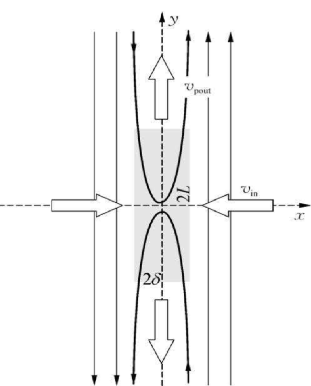
\includegraphics[width=0.4\textwidth]{figures/磁重联简介-2.pdf}
	\end{center}
	
	上面这个模型可以直接放到GR框架下，只需要把方程在电流片的local rest frame（LRF）下展开计算。Asenjo和Comisso在2017年考虑电流片的LRF就是ZAMO系，并进行计算。尽管这并不合理，但其做法仍具有指导意义。下面我们简单介绍一下。
	
	为了使解析计算能做下去，我们需要进行一些简化和假设。首先，我们假设该模型在BL坐标系下是稳态的，即$\partial_t \approx 0$。其次，由于磁重联给磁流体提供了足够大的动能，我们认为电流片的出射速度远大于黑洞旋转速度，即$\hat{v}_{\text{out}} \gg \beta^{\phi}$。最后，由于磁重联尺度非常小（介观尺度），当电流片离黑洞足够远时，与度规有关的导数项可以忽略，即$G_{ij} \approx \sigma_{ij} \approx 0$，$\partial_j h_i \approx 0$。由于黑洞附近的磁重联主要发生在赤道面附近的吸积盘中，因此我们就将电流片至于赤道面上（$\theta = \pi / 2$），于是有$\partial_{\theta} = 0$。
	
	作为一个示例，我们考虑电流片躺在赤道面上，长边沿着$\phi$方向，设其在BL系下的长度为$2L$，短边沿着$r$方向，设其在BL系下长度为$2\delta$。在电流片上流方向的流入点，磁场大小是一个常数，记为$\hat{B}_0$，方向沿着$\phi$方向。电流片的中心记作$X$点，沿着电流片长边过$X$点的线称为中心线。在中心线上：（1）流入的磁流体$r$方向速度消失（$\hat{v}^r = 0$），之后沿着$\phi$方向被加速直到下游的流出点；（2）原本$\phi$方向的磁力线也在此处因重联而消失（$\hat{B}^{\phi} = 0$）, 而在下游流出点，被磁流体带出的重联后的磁场方向为$r$方向，大小记作$\hat{B}_{\text{out}}$；（3）电流为$\theta$方向，且在整个电流片均匀分布，电荷密度为0。我们先看在流出点的磁场，由磁通量守恒：（严格来说，磁通量并不守恒，但可用于估算）
	\begin{equation}
		\hat{B}_0 \hat{\delta} \approx \hat{B}_{\text{out}} \hat{L}
	\end{equation}
	其中$\hat{\delta} = h_1 \delta$，$\hat{L} = \frac{h_3}{r} L$为固有长度或者说坐标长度（实际上，后面所有的计算只不过是将原本LRF的结果中的固有长度换成这里定义的BL系的长度，最后的引力修正实际上也源于此）。于是我们得到：（该关系也可由磁场散度为0得到）
	\begin{equation}
		\hat{B}_{\text{out}} \approx \left( \frac{r h_1}{h_3} \right) \frac{\delta}{L} \hat{B}_0
	\end{equation}
	可以看到，重联后的磁场远远小于重联前的磁场。
	
	我们设在LRF下（ZAMO系），流入的磁流体4-速为：
	\begin{equation}
		\hat{u}_{\text{in}} = \hat{\gamma}_{\text{in}} (1, \hat{v}_{\text{in}}, 0, 0)
	\end{equation}
	流出的磁流体4-速为：
	\begin{equation}
		\hat{u}_{\text{out}} = \hat{\gamma}_{\text{out}} (1, 0, 0, \hat{v}_{\text{out}})
	\end{equation}
	我们也可以计算出BL系下的4-速：
	\begin{equation}
		u_{\text{in}} = \hat{\gamma}_{\text{in}} \left( \frac{1}{\alpha}, \frac{\hat{v}_{\text{in}}}{h_1}, 0, 0 \right)
	\end{equation}
	\begin{equation}
		u_{\text{out}} = \hat{\gamma}_{\text{out}} \left( \frac{1}{\alpha}, 0, 0, \frac{\hat{v}_{\text{out}} + \beta^{\phi}}{h_3} \right)
	\end{equation}
	在中心线上，由能量动量守恒方程：
	\begin{equation}
		\frac{1}{h_1 h_2 h_3} \sum_{j = 1}^3 \frac{\partial}{\partial x^j} \left[ \frac{\alpha h_1 h_2 {h_3} }{h_j} (h \hat{\gamma}^2 \hat{v}^i \hat{v}^j + \beta^j h \hat{\gamma}^2 \hat{v}^i) \right] + \frac{h \hat{\gamma}^2}{h_i} \frac{\partial \alpha}{\partial x^i} = \alpha (- \partial^i p_g + \hat{J}^j \hat{F}^i{}_j)
	\end{equation}
	由前面的假设和简化，我们得到：
	\begin{equation}
		\partial_{\phi} [h \hat{\gamma}^2 (\hat{v}^{\phi})^2] = - \partial_{\phi} p_g - h_3 \hat{J}^{\theta} \hat{B}^r
	\end{equation}
	由于中心点$X$处的磁流体压强要与上游的磁压平衡，于是有$p_{g,X} = \hat{B}^2_0 / 2$。由安培定律，电流密度是入流磁场的旋度（实际上有两项，只不过出流的磁场太弱，忽略这一项），即：
	\begin{equation}
		\hat{J}^{\theta} \approx - \frac{\hat{B}_0}{\hat{\delta}} = - \frac{1}{h_1} \frac{\hat{B}_0}{\delta}
	\end{equation}
	考虑这些边界条件后，我们可以对能量动量守恒方程从$X$点积到流出点，得到：（整一段的磁场取平均）
	\begin{equation}
		\hat{\gamma}_{\text{out}} \hat{v}_{\text{out}} \approx \frac{1}{\sqrt{2}}
	\end{equation}
	这其实就是在GR框架下，上游磁场$\hat{B}_0$决定的Alfvén速度，只不过这里采用了相对论性的热等离子体假设（$h \approx 4 p_g$），于是有这么一个确切的数值。总之，磁流体经过磁重联过程后，会被加速到Alfvén速度这样一个相当快的速度（光速的量级），于是整个重联速率完全取决于磁流体流入电流片的速度（来多少加速多少）。
	
	\begin{center}
		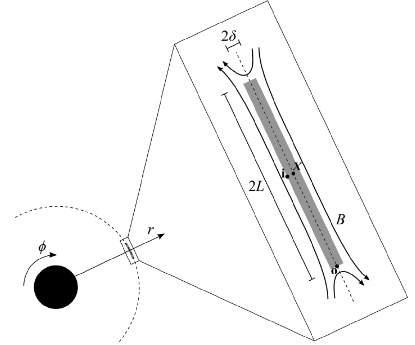
\includegraphics[width=0.5\textwidth]{figures/磁重联简介-3.pdf}
	\end{center}
	
	接着我们考虑入流速度。我们先看电磁张量中，所有非零分量：
	\[ F^{02} = - F^{20} = \frac{1}{\alpha h_2} \hat{E}^{\theta}, \quad F^{12} = - F^{21} = \frac{1}{h_1 h_2} \hat{B}^{\phi}, \quad F^{23} = - F^{32} = \frac{1}{h_2 h_3} (\hat{B}^r + \beta^{\phi} \hat{E}^{\theta}) \]
	由无源麦克斯韦方程：
	\begin{equation}
		\frac{1}{\alpha h_1 h_2 h_3} \partial_j (\alpha h_1 h_2 h_3 {}^{*}F^{\mu \nu}) = 0
	\end{equation}
	可得$\partial_r (\alpha h_2 \hat{E}^{\theta}) = 0$，即电流片内的电场沿着$r$方向均匀分布（这段分析其实完全可以在LRF下利用法拉第电磁感应定律得到）。根据欧姆定律：
	\begin{equation}
		\hat{F}^{\mu \nu} \hat{u}_{\nu} = \eta \hat{J}^{\mu}
	\end{equation}
	即：
	\begin{equation}
		\hat{\gamma} \hat{E}^{\theta} + \hat{\gamma} \hat{v}^{\phi} \hat{B}^r = \eta \hat{J}^{\theta}
	\end{equation}
	在$X$点，电场为：
	\begin{equation}
		\hat{E}^{\theta} |_X = \eta \hat{J}^{\theta}
	\end{equation}
	在流入点，电场为：
	\begin{equation}
		\hat{E}^{\theta} |_{\text{in}} = \hat{v}_{\text{in}} \hat{B}_0
	\end{equation}
	由$\hat{E}^{\theta} |_X = \hat{E}^{\theta} |_{\text{in}}$，我们得到：
	\begin{equation}
		\hat{v}_{\text{in}} = \frac{\eta}{h_1 \delta}
	\end{equation}
	接下来我们需要计算$\delta$。考虑质量守恒方程：
	\begin{equation}
		\frac{1}{\alpha h_1 h_2 h_3} \partial_{\mu} (\alpha h_1 h_2 h_3 \rho u^{\mu}) = 0
	\end{equation}
	我们可以得到流入的通量为$\frac{1}{\alpha h_1 h_2 h_3} \partial_r \left( \alpha h_1 h_2 h_3 \rho \frac{\hat{\gamma} \hat{v}^r}{h_1} \right) \approx \frac{\rho \hat{\gamma}_{\text{in}} \hat{v}_{\text{in}}}{h_1 \delta}$，流出的通量为$\frac{1}{\alpha h_1 h_2 h_3} \partial_{\phi} \left( \alpha h_1 h_2 h_3 \rho \frac{\hat{\gamma} \hat{v}^{\phi}}{h_3} \right) \approx \frac{\rho \hat{\gamma}_{\text{out}} \hat{v}_{\text{out}}}{h_3 L / r}$，于是有：
	\begin{equation}
		\delta \approx \frac{h_3}{h_1 r} \frac{\hat{\gamma}_{\text{in}} \hat{v}_{\text{in}}}{\hat{\gamma}_{\text{out}} \hat{v}_{\text{out}}} L
	\end{equation}
	忽略流入磁流体的洛伦兹因子（$\hat{\gamma}_{\text{in}} \approx 1$），于是我们得到重联速率：
	\begin{equation}
		\hat{v}_{\text{in}} \approx S^{- 1 / 2} \sqrt{\frac{r_o}{h_3 |_o}}
	\end{equation}
	其中，$S = L / \eta$称为Lundquist数（其实就是磁雷诺数）。我们将$h_3 = \sqrt{r^2 + a^2 + \frac{2 a^2}{r}}$代入，并取$r_o \gg 1$近似，可得：
	\begin{equation}
		\hat{v}_{\text{in}} \approx S^{- 1 / 2} \left( 1 - \frac{a^2}{4 r^2_o} \right)
	\end{equation}
	可见Kerr时空下，该位形的磁重联速率会降低。这表明在特定位形下，黑洞的参考系拖拽效应起到了抑制作用，使得磁力线更难被带入耗散区。
	
	尽管在空间和高能天体等离子体中，磁雷诺数很大，但Sweet-Parker模型仍不能解释高能天体中磁场能量快速释放的事件（时间尺度相差3个量级）。Sweet-Parker模型的瓶颈在于，一方面我们要求电流片宽度$\delta$足够小，使得入流速度足够大；可另一方面，由质量守恒要求，宽度$\delta$越小，出流流体越少，这使得沿长边$L$入流流体速度不能太大，从而限制了重联率。
	
	\section{Petschek模型}
	
	为了解决Sweet-Parker模型重联速率的瓶颈，Petschek于1963年提出了二维稳态快重联模型，我们称为Petschek模型。我们可以将Petschek模型分为流入区、中心耗散区、流出区和慢激波（也成为边界层）这4个部分。流入区在远离中心耗散区的地方与Sweet-Parker模型一样，磁场是均匀的，流体以一个较慢的速度流向中心。但不同于Sweet-Parker模型中的平直磁力线位形，Petschek模型中磁场位形要求进入电流片（由于激波面内也存在电流，因此这里的电流片包括中心耗散区和向外延伸的慢激波）中心附近的磁力线是弯曲的，因此实际的耗散区域长度远小于$2L$。中心耗散区等同于一个微型的Sweet-Parker电流片，其作用主要是重联磁场，改变磁场的拓扑结构。绝大部分的磁场能量到磁流体动能的转换，则发生在从这个中心耗散区向外延伸的慢激波上。这个结构性的改变，使得磁流体和磁力线可以从一个更宽的区域流入，从而极大地提高了整体的重联速率。慢激波是流入区与流出区的边界，其宽度（即电流片的宽度）是变化的。穿过激波，磁场和磁流体速度会发生跃变，但仍然遵守质量守恒、能量动量守恒、总压强守恒以及切向电场与法向磁场的连续性。
	
	Petschek模型的基本假设有：（1）稳态模型，物理量对时间偏微分为零，即$\partial_t \approx 0$，根据法拉第电磁感应定律，这也就导致电场在电流片中均匀分布；（2）入流区磁场$\vec{B}_{\text{in}}$相对于上游的磁场$\vec{B}_0$的偏离是一阶小量，即$\vec{B}_{\text{in}} = \vec{B}_0 + \vec{B}_1, | B_1 | \ll | B_0 |$，边界层的入流速度相对于$B_0$决定的Alfvén速度是一阶小量；（3）电流严格限制于耗散区和边界层内，流入区的磁场是势场，可以由边界条件给出。最后，Petschek模型的解析解是半定量的，我们忽略具体复杂的电流片结构，边界层中的物理量是沿电流片宽度积分的平均解。
	
	\begin{center}
		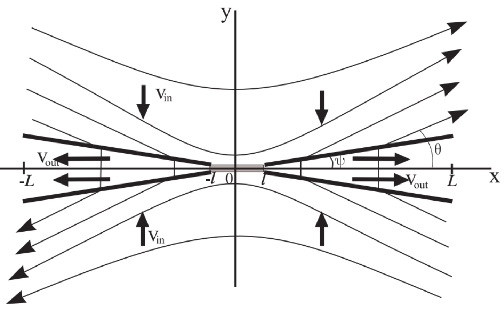
\includegraphics[width=0.6\textwidth]{figures/磁重联简介-4.pdf}
	\end{center}
	
	该模型也可以直接放到GR框架下进行计算，该工作由范仲英老师首次完成，下面我们简单介绍一下。作为示例，我们同样考虑电流片作为ZAMO观者躺在赤道面上的情况。电流片的中心为$C$点，我们定义电流片LRF坐标为$x = r - r_C, y = h_3 \phi / r_C$。中心扩散区长度和宽度在BL系下分别为$2Y$和$2X$，电流片的长度在BL系下为$2L$，且$L \gg Y$，电流片宽度是坐标$y$的函数$2 \Delta(y)$。ZAMO系下流入区域的磁场设为$\hat{\bm{B}}_{\text{in}} = - \hat{B}_0 \bm{e}_{\phi} + \hat{\bm{B}}_1$，且$| \hat{\bm{B}}_1 | \ll \hat{B}_0$。在中心扩散区，重联率仍是Sweet-Parker模型计算结果：
	\begin{equation}
		M \approx \frac{h_1 X}{Y} \approx \left( \frac{Y h_3}{\eta r} \right)^{- 1 / 2}
	\end{equation}
	耗散区的宽度：
	\begin{equation}
		X \approx \frac{\eta}{h_1 \hat{v}_i}
	\end{equation}
	\begin{center}
		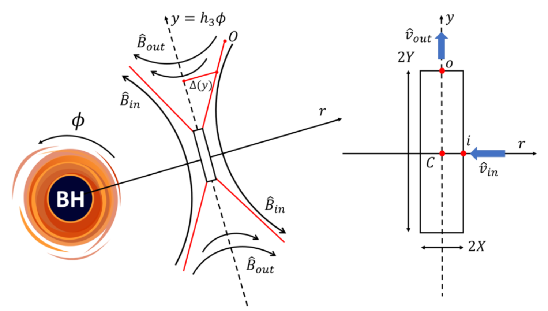
\includegraphics[width=0.7\textwidth]{figures/磁重联简介-5.pdf}
	\end{center}
	
	之前的假设仍然成立，即$\partial_t \approx 0$，$\hat{v}_{\text{out}} \gg \beta^{\phi}$，$G_{ij} \approx \sigma_{ij} \approx 0$，$\partial_j h_i \approx 0$以及$\partial_{\theta} = 0$。耗散区及边界层的电流和电场设为$\bm{J} = \hat{J}^{\theta} \bm{e}_{\theta}$和$\bm{E} = \hat{E}^{\theta} \bm{e}_{\theta}$，磁流体流入点速度为$\hat{\bm{v}}_{\text{in}} = - \hat{v}_i \bm{e}_r$。我们考虑边界层上任意一点$O$，该点的电流片厚度可由质量守恒给出，流入的通量大约为$\rho \hat{\gamma}_i \hat{v}_i / (h_1 \Delta)$，流出的通量大约为$\rho \hat{\gamma}_o \hat{v}_o / y$，于是有：
	\begin{equation}
		\Delta (y) \approx \frac{\hat{\gamma}_i \hat{v}_i}{\hat{\gamma}_o \hat{v}_o} \frac{y}{h_1}
	\end{equation}
	电流片内的欧姆定律仍然是：
	\begin{equation}
		\hat{\gamma} \hat{E}^{\theta} + \hat{\gamma} \hat{v}^{\phi} \hat{B}^r = \eta \hat{J}^{\theta}
	\end{equation}
	由于电场均匀分布，我们只须计算一处的电场。在流入点，电场为：
	\begin{equation}
		\hat{E}^{\theta} |_i = \hat{v}_i \hat{B}_0
	\end{equation}
	$O$点的电场$\hat{E}^{\theta} |_O = \hat{E}^{\theta} |_i$。而$O$点的电流可由麦克斯韦方程计算：
	\begin{equation}
		\hat{J}^{\theta} |_O \approx h^{- 1} \partial_r \hat{F}^{\theta r} \approx \frac{\hat{B}_0}{h_1 \Delta (y)}
	\end{equation}
	于是我们得到：
	\begin{equation}
		\Delta (y) - \frac{\hat{\gamma}_i \hat{B}_O}{\hat{\gamma}_O \hat{B}_0} \frac{y}{h_1} - \frac{\eta}{\hat{\gamma}_O \hat{v}_i h_1} = 0
	\end{equation}
	在靠近中心耗散区的位置，第二项可以忽略，于是$\Delta \approx \eta / (\hat{v}_i h_1) \approx X$；而在远离中心的区域，及$y \approx L$，第三项可以忽略，于是：
	\begin{equation}
		\left( \frac{h_1 \Delta (y)}{y} \right)_{y \approx L} \approx \frac{\hat{\gamma}_i \hat{B}_O}{\hat{\gamma}_O \hat{B}_0}
	\end{equation}
	结合质量守恒方程，我们得到：
	\begin{equation}
		\hat{v}_i \approx \frac{\hat{B}_O}{\hat{B}_0} \approx \frac{h_1 \Delta (y)}{y}
	\end{equation}
	即边界层在远离中心区域近似一条直线，斜率正比于$\hat{v}_i$。由$\phi$方向能量动量守恒方程：
	\begin{equation}
		\partial_y [h \hat{\gamma}^2 (\hat{v}^{\phi})^2] + \partial_r (h_1^{- 1} h \hat{\gamma}^2 \hat{v}^r \hat{v}^{\phi}) = - \frac{\partial p}{\partial y} - \hat{J}^{\theta} \hat{B}^r
	\end{equation}
	沿径向积分得到：
	\begin{equation}
		\frac{\hat{B}_O}{\hat{B}_0} \approx \frac{h \hat{v}_i^2}{\hat{B}^2_0} \left[ 2 y \partial_y \left( \frac{y}{h_1 \Delta (y)} \right) + \frac{\hat{\gamma}_O y}{h_1 \Delta (y)} \right]
	\end{equation}
	整理可得：
	\begin{equation}
		h_1 \Delta (y) - 2 \hat{v}^2_i y \left[ 2 \hat{\gamma}_O^{- 1} y \partial_y \left( \frac{y}{h_1 \Delta (y)} \right) + \frac{y}{h_1 \Delta (y)} \right] - \frac{\eta}{\hat{\gamma}_O \hat{v}_i} = 0
	\end{equation}
	该方程给出了电流片宽度$\Delta$随坐标$y$的变化关系。能量动量守恒方程沿$y$方向从$C$点积分到$O$点，得到：
	\begin{equation}
		h \left( \hat{\gamma}^2_O \hat{v}_O^2 + \hat{\gamma}^2_O \hat{v}_O \hat{v}_i \frac{y}{h_1 \Delta (y)} \right) = p \left( 1 + \frac{2 y}{h_1 \Delta (y)} \frac{\hat{B}_O}{\hat{B}_0} \right)
	\end{equation}
	结合上面的方程，该方程给出出射速度$\hat{v}_O$随坐标$y$的变化关系。可以看到，在远离中心区域：
	\begin{equation}
		(\hat{\gamma}^2_O \hat{v}_O^2 + \hat{\gamma}^2_O \hat{v}_O)_{y \approx L} \approx \frac{3}{4}
	\end{equation}
	即$\hat{\gamma}_O \hat{v}_O |_{y \approx L} \approx 1 / 2$。
	
	现在我们考虑如何求解入流区的磁场偏离$\hat{\bm{B}}_1$。由于其为势场，可以由边界条件完全决定。由于边界面的夹角比较小，可以近似为0，即$x=0$的平面，则$\hat{\bm{B}}_1$可以看作是由边界面上的磁单极子$B_{1 \bot} \approx \mp 2 \hat{v}_i \hat{B}_0$产生的势场。通过格林函数的方法可计算出流入点的磁场偏离：
	\begin{equation}
		\hat{B}_1^{\phi} |_i \approx \frac{2 \hat{v}_i \hat{B}_0}{\pi} \ln \left( \frac{L^2}{Y^2} \right) \approx \frac{4 \hat{v}_i \hat{B}_0}{\pi} \ln \left( \hat{v}_i^2 S \frac{h_3 (r_O)}{r_O} \right)
	\end{equation}
	于是：
	\begin{equation}
		\hat{v}_i \approx k \left( \ln \left( \hat{v}_i^2 S \frac{h_3 (r_O)}{r_O} \right) \right)^{- 1}, \quad k = \frac{\pi \hat{B}^{\phi}_1 |_i}{4 \hat{B}_0 |_i}
	\end{equation}
	展开后得到：
	\begin{equation}
		\hat{v}_i \approx k \left[ \ln (\hat{v}_i^2 S) + \frac{a^2}{2 r^2_O} \right]^{- 1}
	\end{equation}
	
	\section{无碰撞模型}
	
	前面我们提到，在高能天体环境中，等离子体处于高温、低密度状态，粒子之间的碰撞频率极低，平均自由程远大于系统的特征尺度，因此基于碰撞的电阻率几乎为零。在这种情况下，我们需要考虑其他机制来打破磁冻结机制，而无碰撞磁重联模型正是为了解决这一问题而生。该模型的核心思想是：当尺度小到一定程度时，单流体MHD描述失效，离子和电子的运动会发生解耦。这种双流体效应或纯粹的粒子动理学效应，提供了新的机制，如霍尔效应、电子惯性和电子压力张量的非对角项等耗散机制，来打破磁冻结，从而实现快速重联。这一模型最早由Koide推广到GR框架下，Asenjo和Comisso完成了GR框架下的解析计算，下面我们介绍一下。请注意，下面所展示的内容忽略了霍尔效应，仅考虑了电子的热效应。而实际上，霍尔效应也扮演着非常重要的角色。
	
	无碰撞模型的基本方程有：
	
	（1）质量守恒方程：
	\begin{equation}
		\nabla_{\mu} (n U^{\mu}) = 0
	\end{equation}
	（2）能量动量守恒方程：
	\begin{equation}
		\nabla_{\nu} \left[ p g^{\mu \nu} + h \left( U^{\mu} U^{\nu} + \frac{\xi}{4 n^2 e^2} J^{\mu} J^{\nu} \right) + F^{\mu \sigma} F^{\nu}{}_{\sigma} - \frac{1}{4} g^{\mu \nu} F^2 \right] = 0
	\end{equation}
	其中，$e$是电子电荷，$h = n^2 (h_+ / n_+^2 + h_- / n_-^2)$是固有系下的焓密度，$p = p_+ + p_-$是固有系下的压强，$\xi$满足：
	\begin{equation}
		\xi = 1 - \mu^2
	\end{equation}
	其中：
	\begin{equation}
		\mu = \frac{m_+ - m_-}{m_+ + m_-}
	\end{equation}
	表示正负带点粒子质量差异。这里我们只考虑$\mu = 0$的情况。
	
	（3）麦克斯韦方程：
	\begin{equation}
		\nabla_{\mu} F^{\mu \nu} = - J^{\nu}, \quad \nabla_{\nu} {}^{*}F^{\mu \nu} = 0
	\end{equation}
	（4）广义欧姆定律：（忽略霍尔效应项）
	\begin{equation}
		U^{\nu} F^{\mu}{}_{\nu} = \eta (J^{\mu} - \rho_e U^{\mu}) + \frac{1}{n e} \nabla_{\nu} \left[ \frac{\xi h}{4 n e} \left( U^{\mu} J^{\nu} + J^{\mu} U^{\nu} - \frac{\mu}{n e} J^{\mu} J^{\nu} \right) \right]
	\end{equation}
	右边多出来的这一项正是电子热效应带来的耗散项。
	
	将这些方程在ZAMO系展开：
	
	（1）质量守恒方程：
	\begin{equation}
		\frac{\partial}{\partial t} (n \hat{\gamma}) + \frac{1}{h_1 h_2 h_3} \sum_j \partial_j \left( \frac{\alpha h_1 h_2 h_3}{h_j} n \hat{\gamma} (\hat{v}^j + \beta^j) \right) = 0
	\end{equation}
	（2）能量动量守恒方程：
	\begin{multline}
		\partial_t \hat{P}^i + \frac{1}{h_1 h_2 h_3} \sum_j \partial_j \left[ \frac{\alpha h_1 h_2 h_3}{h_j} ( \hat{T}^{i j} + \beta^j \hat{P}^i) \right] + \frac{\varepsilon + \hat{\gamma} \rho}{h_i} \partial_i \alpha \\
		- \alpha \sum_j [(G_{i j} \hat{T}^{i j} - G_{j i} \hat{T}^{j j}) - (\beta^i G_{i j} - \beta^j G_{j i}) \hat{P}^j] + \sum_j \sigma_{j i} \hat{P}^j = 0
	\end{multline}
	其中：
	\begin{equation}
		\varepsilon = - p + h \hat{\gamma}^2 + \frac{h \xi}{4 n^2 e^2} (\hat{J}^0)^2 + \frac{1}{2} (\hat{E}^2 + \hat{B}^2) - \hat{\gamma} \rho
	\end{equation}
	\begin{equation}
		\hat{P}^i = h \hat{\gamma}^2 \hat{v}^i + \frac{h \xi}{4 n^2 e^2} \hat{J}^i \hat{J}^0 + \sum_{j, k} \epsilon^{i j k} \hat{E}^j \hat{B}^k
	\end{equation}
	\begin{equation}
		\hat{T}^{i j} = p \delta^{i j} + h \hat{\gamma}^2 \hat{v}^i \hat{v}^j + \frac{h \xi}{4 n^2 e^2} \hat{J}^i \hat{J}^j - \hat{E}^i \hat{E}^j - \hat{B}^i \hat{B}^j + \frac{1}{2} (\hat{E}^2 + \hat{B}^2) \delta^{i j}
	\end{equation}
	（3）麦克斯韦方程：
	\begin{equation}
		\sum_j \partial_j \left( \frac{h_1 h_2 h_3}{h_j} \hat{B}^j \right) = 0
	\end{equation}
	\begin{equation}
		\frac{1}{h_1 h_2 h_3} \sum_j \partial_j \left( \frac{h_1 h_2 h_3}{h_j} \hat{E}^j \right) = \hat{J}^0
	\end{equation}
	\begin{equation}
		\alpha (1 + \beta^i) \hat{J}^i + \partial_t \hat{E}^i = \frac{h_i}{h_1 h_2 h_3} \sum_{j, k} \partial_j \left[ \frac{\alpha h_1 h_2 h_3}{h_i h_j} (\epsilon^{i j k} \hat{B}^k + \beta^i \hat{E}^j - \beta^j \hat{E}^i) \right]
	\end{equation}
	\begin{equation}
		\partial_t \hat{B}^i = \frac{h_i}{h_1 h_2 h_3} \sum_{j, k} \partial_j \left[ \frac{\alpha h_1 h_2 h_3}{h_i h_j} (\epsilon^{i j k} \hat{E}^k + \beta^i \hat{B}^j - \beta^j \hat{B}^i) \right]
	\end{equation}
	（4）广义欧姆定律：
	\begin{multline}
		\frac{1}{n e} \partial_t \hat{K}^{00} + \frac{1}{n e h_1 h_2 h_3} \sum_j \partial_j \left( \frac{\alpha h_1 h_2 h_3}{h_j} (\hat{K}^{0 j} + \beta^j \hat{K}^{00}) \right) + \frac{1}{n e} \sum_j \frac{\partial_j \alpha}{h_j} \hat{K}^{0 j} \\
		+ \frac{\alpha}{n e} \sum_{j, k} \beta^k [G_{k j} (\hat{K}^{k j} + 2 \beta^j \beta^k \hat{K}^{00}) - G_{j k} (\hat{K}^{j j} + 2 (\beta^j)^2 \hat{K}^{00})] \\
		+ \frac{1}{n e} \sum_{j, k} \sigma_{j k} (\hat{K}^{j k} + 2 \beta^j \beta^k \hat{K}^{00}) = \alpha \hat{H}^0
	\end{multline}
	\begin{multline}
		\frac{1}{n e} \partial_t \hat{K}^{0 i} + \frac{1}{n e h_1 h_2 h_3} \sum_j \partial_j \left( \frac{\alpha h_1 h_2 h_3}{h_j} (\hat{K}^{i j} + \beta^j \hat{K}^{0 i}) \right) + \frac{\hat{K}^{00}}{n e h_i} \partial_i \alpha \\
		- \frac{\alpha}{n e} \sum_j \partial_j [G_{i j} (\hat{K}^{i j} + \beta^j \hat{K}^{0 i}) - G_{j i} (\hat{K}^{j j} + \beta^j \hat{K}^{0 j})] + \frac{1}{n e} \sum_j \sigma_{j i} \hat{K}^{0 j} = \alpha \hat{H}^i
	\end{multline}
	其中：
	\begin{equation}
		\begin{aligned}
			\hat{K}^{00} & = \frac{h \xi \hat{\gamma}}{2 n e} \hat{J}^0\\
			\hat{K}^{0 i} & = \frac{h \xi \hat{\gamma}}{4 n e} (\hat{J}^i + \hat{J}^0 \hat{v}^i)\\
			\hat{K}^{i j} & = \frac{h \xi \hat{\gamma}}{4 n e} (\hat{v}^i \hat{J}^j + \hat{v}^j \hat{J}^i)\\
			\hat{H}^0 & = \hat{\gamma} \hat{v}^i \hat{E}_i + \eta \hat{\gamma}^2 \hat{v}^2 \hat{J}^0\\
			\hat{H}^i & = \hat{\gamma} \left( \hat{E}^i + \sum_{j, k} \epsilon^{i j k} \hat{v}_j \hat{B}_k \right) - \eta (\hat{J}^i - \rho_e \hat{\gamma} \hat{v}^i)
		\end{aligned}
	\end{equation}
	\begin{center}
		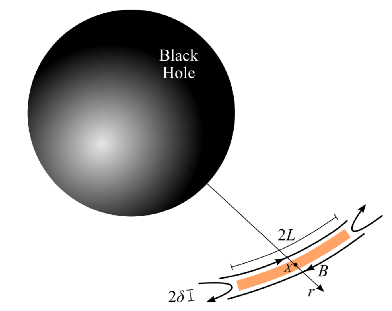
\includegraphics[width=0.5\textwidth]{figures/磁重联简介-6.pdf}
	\end{center}
	
	作为示例，我们考虑电流片作为ZAMO观者躺在赤道面上的情况。整个计算基本与Sweet-Parker模型无异，其基本假设我们不再赘述。由磁通量守恒可得：
	\begin{equation}
		\hat{B}_{\text{out}} \approx \left( \frac{r h_1}{h_3} \right) \frac{\delta}{L} \hat{B}_{\text{in}}
	\end{equation}
	在电流片中心线上，能量动量守恒方程给出：
	\begin{equation}
		\partial_{\phi} \left[ h \hat{\gamma}^2 (\hat{v}^{\phi})^2 - \frac{\hat{B}^2}{2} + p \right] = 0
	\end{equation}
	假设流出的是相对论性热的磁流体（$h = 4 p$），加上中心气压与流入点的磁压平衡（$p = \hat{B}^2_{\text{in}} / 2$），我们可以得到：
	\begin{equation}
		\hat{\gamma}_{\text{out}} \hat{v}_{\text{out}} = \frac{1}{\sqrt{2}}
	\end{equation}
	质量守恒则给出：
	\begin{equation}
		\delta \approx \frac{h_3}{h_1 r} \frac{\hat{\gamma}_{\text{in}} \hat{v}_{\text{in}}}{\hat{\gamma}_{\text{out}} \hat{v}_{\text{out}}} L
	\end{equation}
	无碰撞与Sweet-Parker模型不同之处在于广义欧姆定律。在流入点，电场仍为：
	\begin{equation}
		\hat{E}^{\theta} |_{\text{in}} = \hat{v}_{\text{in}} \hat{B}_{\text{in}}
	\end{equation}
	而在$X$点，$\theta$方向的广义欧姆定律：
	\begin{equation}
		\frac{1}{n e} \sum_j \partial_j \left( \frac{1}{h_j} \hat{K}^{\theta j} \right) = \hat{H}^{\theta}
	\end{equation}
	可得：
	\begin{equation}
		\hat{E}^{\theta} |_X \approx (\eta + \Lambda) \hat{J}^{\theta} |_X
	\end{equation}
	其中：
	\begin{equation}
		\Lambda = \frac{h \xi}{4 n^2 e^2 L} \frac{r}{h_3} \hat{\gamma}_{\text{out}} \hat{v}^{\phi}_{\text{out}} \approx \frac{h \xi}{4 n^2 e^2 L} \frac{r}{h_3}
	\end{equation}
	是电子热效应提供的等效电阻率，引力修正项：
	\begin{equation}
		\frac{r}{h_3} \approx 1 - \frac{a^2}{2 r^2_X}
	\end{equation}
	电流可由磁场旋度计算：
	\begin{equation}
		\hat{J}^{\theta} |_X \approx - \frac{\hat{B}_{\text{in}}}{h_1 \delta}
	\end{equation}
	由$\hat{E}^{\theta} |_{\text{in}} = \hat{E}^{\theta} |_X$，我们得到：
	\begin{equation}
		\hat{v}_{\text{in}} \approx \sqrt{\frac{r}{h_3} \left( S^{- 1} + \frac{\Lambda}{L} \right)}
	\end{equation}
	可见，无碰撞效应能提高重联率。
	
	\chapter{磁重联成像}
	
	\section{磁重联与热点成像}
	由于磁重联事件能快速释放磁场中的能量，并转化为磁流体的动能和内能，因此这一机制可以作为热点模型的候选者，从而被我们的望远镜捕捉。此外，由于磁重联事件能使磁流体加速到接近光速，当这一事件发生在黑洞能层内时，其可以作为彭罗斯过程的点火机制，从而实现提取黑洞的旋转能量。这一提取黑洞能量的机制由Asenjo和Comisso完成，而磁重联彭罗斯过程（Magnetic Reconnection Penrose Process, MRPP）这一事件的热点成像由我们组内的赵之星师姐完成，下面我们简单介绍一下。
	
	前面我们重点关注的是此重联速率的快慢。现在我们在Petschek模型的基础上，重点关注从电流片出来的磁流体速度最大能达到多少。如下图所示，在流入区，磁流体压强以磁压为主，气压可以忽略。以下所有分析都是在电流片的LRF下进行的。
	
	\begin{center}
		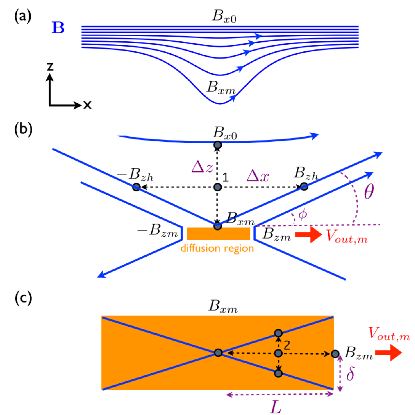
\includegraphics[width=0.5\textwidth]{figures/磁重联简介-7.pdf}
	\end{center}
	
	在point 1处，由磁流体静力学，磁压梯度力$- (\vec{\nabla} B^2 / 2)_z$与磁张力$\vec{B} \cdummy \vec{\nabla} B_z$平衡，于是有：（这里假定磁场是均匀变化的）
	\begin{equation}
		\frac{B_{x 0}^2 - B^2_{x m}}{2 \Delta z} \approx \left( \frac{B_{x 0} + B_{x m}}{2} \right) \frac{2 B_{z h}}{\Delta x}
	\end{equation}
	解出：
	\begin{equation}
		\frac{\Delta z}{\Delta x} \approx \frac{B_{x 0} - B_{x m}}{2 B_{z h}}
	\end{equation}
	从几何的角度考虑，假设：
	\begin{equation}
		\frac{\Delta z}{\Delta x} \approx \frac{B_{z h}}{(B_{x 0} + B_{x m}) / 2}
	\end{equation}
	上面两式消去$B_{z h}$，得到：
	\begin{equation}
		\frac{B_{x m}}{B_{x 0}} \approx \frac{1 - (\Delta z / \Delta x)^2}{1 + (\Delta z / \Delta x)^2}
	\end{equation}
	此外，我们假设张角有以下关系：（$\theta \approx \phi$）
	\begin{equation}
		\frac{\Delta z}{\Delta x} \approx \frac{B_{z m}}{B_{x m}} \approx \frac{\delta}{L}
	\end{equation}
	在point 2处，考虑能量动量守恒：
	\begin{equation}
		\partial_{\mu} T^{\mu \nu} = 0
	\end{equation}
	的$x$分量。其中：
	\begin{equation}
		T^{\mu \nu} = h u^{\mu} u^{\nu} + p \eta^{\mu \nu} + F^{\mu \rho} F^{\nu}{}_{\rho} - \frac{1}{4} \eta^{\mu \nu} F^{\rho \sigma} F_{\rho \sigma}
	\end{equation}
	\begin{equation}
		u^{\mu} = \gamma_{\text{out}} (1, v_{\text{out}}, 0, 0)
	\end{equation}
	于是：（$p = B^2 / 2$）
	\begin{equation}
		T^{x x} = h \gamma_{\text{out}}^2 v_{\text{out}}^2 + B^2_{z m}
	\end{equation}
	\begin{equation}
		T^{z x} = - B_{z m} B_{x m}
	\end{equation}
	于是能量动量守恒给出：
	\begin{equation}
		h \gamma_{\text{out}}^2 v_{\text{out}}^2 / L + B^2_{z m} / L - B_{z m} B_{x m} / \delta \approx 0
	\end{equation}
	解得：
	\begin{equation}
		v_{\text{out}} \approx \sqrt{\frac{(1 - \delta^2 / L^2) \sigma_{x m}}{1 + (1 - \delta^2 / L^2) \sigma_{x m}}}
	\end{equation}
	其中：
	\begin{equation}
		\sigma_{x m} = B^2_{x m} / h = \left( \frac{1 - (\Delta z / \Delta x)^2}{1 + (\Delta z / \Delta x)^2} \right)^2 B^2_{x 0} / h \equiv \left( \frac{1 - (\Delta z / \Delta x)^2}{1 + (\Delta z / \Delta x)^2} \right)^2 \sigma_0
	\end{equation}
	即：
	\[ v_{\text{out}} \approx \sqrt{\frac{(1 - \delta^2 / L^2)^3 \sigma_0}{(1 + \delta^2 / L^2)^2 + (1 - \delta^2 / L^2)^3 \sigma_0}} \]
	对于$\delta / L \ll 1$，有：
	\[ v_{\text{out}} \approx \sqrt{\frac{\sigma_0}{1 + \sigma_0}} \]
	即$v_{\text{out}}$达到Alfvén速度。简单分析可知，这也是$v_{\text{out}}$能达到的最大速度。由此可见，最大出射速度取决于上游磁场决定的Alfvén速度。
	
	现在，我们将电流片置于黑洞能层中，并考虑其做开普勒圆轨道运动的情况。开普勒角速度为：
	\begin{equation}
		\Omega_K = \pm \frac{1}{r^{3 / 2} \pm a}
	\end{equation}
	其中$+$表示顺行轨道，$-$表示逆行轨道。这些圆轨道并非都是稳定的，只有当其大于或等于最内稳定圆轨道（Innermost Stable Circular Orbit, ISCO）时，才会稳定绕黑洞运行。ISCO半径为：
	\begin{equation}
		r_{\text{ISCO}} = 3 + Z_2 \mp \sqrt{(3 - Z_1) (3 + Z_1 + 2 Z_2)}
	\end{equation}
	其中：
	\begin{align}
		Z_1 &= 1 + (1 - a^2)^{1 / 3} [(1 + a)^{1 / 3} + (1 - a)^{1 / 3}] \\
		Z_2 &= \sqrt{3 a^2 + Z^2_1}
	\end{align}
	由于电流片置于能层内做开普勒圆轨道，因此只存在顺行轨道。我们可以得到电流片的4速为：
	\begin{equation}
		u_K^{\mu} = u^t_K (1, 0, 0, \Omega_K)
	\end{equation}
	其中：
	\begin{equation}
		u^t_K = \frac{a + r^{3 / 2}}{\sqrt{2 a r^{3 / 2} + r^2 (r - 3)}}
	\end{equation}
	在ZAMO系下，开普勒速度为：
	\begin{equation}
		\hat{v}_K = \frac{\Xi}{\Delta^{1 / 2}} \left( \frac{r^{- 1 / 2} - a r^{-2}}{r^3 - a^2} \right) - \beta^{\phi}
	\end{equation}
	即电流片的4-速为：
	\begin{equation}
		\hat{u}_K = \hat{\gamma}_K (1, 0, 0, \hat{v}_K)
	\end{equation}
	据此，我们建立LRF的4标架：
	\begin{equation}
		\begin{aligned}
			\sigma_0 & = \hat{\gamma}_K (\hat{e}_0 + \hat{v}_K \hat{e}_3) |_{x^i = x^i_o}\\
			\sigma_1 & = \hat{e}_1 |_{x^i = x^i_o}\\
			\sigma_2 & = \hat{e}_2 |_{x^i = x^i_o}\\
			\sigma_3 & = \hat{\gamma}_K (\hat{v}_K  \hat{e}_0 + \hat{e}_3) |_{x^i = x^i_o}
		\end{aligned}
	\end{equation}
	由于电流片的取向可以任意，我们设其与ZAMO标架有一个角度$\xi$。于是通过磁重联加速的等离子体速度可表示为：
	\begin{equation}
		\bm{v}'_{\pm} = \pm v_{\text{out}} (\cos \xi \bm{\sigma}_3 + \sin \xi \bm{\sigma}_1)
	\end{equation}
	其4-速在LRF为：
	\begin{equation}
		{u'}^{\mu} = \gamma_{\text{out}} [\sigma_0^{\mu} \pm v_{\text{out}} (\cos \xi \sigma^{\mu}_3 + \sin \xi \sigma^{\mu}_1)]
	\end{equation}
	在ZAMO系下：
	\begin{equation}
		\hat{u}^{\mu} = \gamma_{\text{out}} [\hat{\gamma}_K (\hat{e}_0^{\mu} + \hat{v}_K \hat{e}_3^{\mu}) \pm v_{\text{out}} (\cos \xi (\hat{\gamma}_K (\hat{v}_K  \hat{e}_0 + \hat{e}_3)) + \sin \xi \hat{e}_1^{\mu})] \equiv \hat{\gamma}_{\text{out}} (1, \hat{v}^r, 0, \hat{v}^{\phi})
	\end{equation}
	其中：
	\begin{align}
		\hat{\gamma}_{\text{out}} &= \gamma_{\text{out}} \hat{\gamma}_K (1 \pm \hat{v}_K v_{\text{out}} \cos \xi) \\
		\hat{v}^r &= \pm \frac{v_{\text{out}} \sin \xi}{\hat{\gamma}_K (1 \pm \hat{v}_K v_{\text{out}} \cos \xi)} \\
		\hat{v}^{\phi} &= \frac{\hat{v}_K \pm v_{\text{out}} \cos \xi}{1 \pm \hat{v}_K v_{\text{out}} \cos \xi}
	\end{align}
	利用能动张量，我们可以计算出射磁流体在ZAMO系下的能量密度：
	\begin{equation}
		\hat{e} = - \hat{P}_t = \hat{T}^{00} = h \hat{\gamma}_{\text{out}}^2 - p + \frac{\hat{B}^2 + \hat{E}^2}{2}
	\end{equation}
	以及角动量：
	\begin{equation}
		\hat{P}_{\phi} = \hat{T}^{03} = h \hat{\gamma}^2_{\text{out}} \hat{v}^{\phi}_{\text{out}} + (\hat{\bm{B}} \times \hat{\bm{E}})^{\phi}
	\end{equation}
	由此可计算BL坐标系下的能量密度（对应于无穷远观者测得的能量密度）：
	\begin{equation}
		e^{\infty} = - P_t = - \frac{\partial \hat{x}^{\nu'}}{\partial x^{\mu}} \hat{P}_{\nu'} = \alpha \hat{e} + \alpha \beta^{\phi} \hat{P}_{\phi}
	\end{equation}
	该能量可分为流体部分和电磁场部分：
	\begin{equation}
		e^{\infty} = e^{\infty}_{\text{hyd}} + e^{\infty}_{\text{em}}
	\end{equation}
	其中：
	\begin{equation}
		e^{\infty}_{\text{hyd}} = \alpha (h \hat{\gamma}_{\text{out}}^2 - p) + \alpha \beta^{\phi} h \hat{\gamma}_{\text{out}}^2 \hat{v}^{(\phi)}_{\text{out}}
	\end{equation}
	\begin{equation}
		e^{\infty}_{\text{em}} = \alpha \frac{\hat{B}^2 + \hat{E}^2}{2} + \alpha \beta^{\phi} (\hat{\bm{B}} \times \hat{\bm{E}})^{(\phi)}
	\end{equation}
	我们假定磁重联过程将大部分电磁场能量转换为流体的动能和内能，因此有$e^{\infty}_{\text{hyd}} \gg e^{\infty}_{\text{em}}$。此外，我们假设出射的等离子体是不可压缩且绝热的，即该过程等离子体能量守恒。因此，相对于无穷远的静止观者，该能量密度相差一个洛伦兹因子，因此有：
	\begin{equation}
		e^{\infty} = \alpha \left[ h (\hat{\gamma}_{\text{out}} + \beta^{\phi} \hat{\gamma}_{\text{out}} \hat{v}^{(\phi)}_{\text{out}}) - \frac{p}{\hat{\gamma}_{\text{out}}} \right]
	\end{equation}
	代入可得：
	\begin{equation}
		e^{\infty}_{\pm} = \alpha \hat{\gamma}_K \left[ h \gamma_{\text{out}} (1 + \hat{v}_K \beta^{\phi}) \pm h \gamma_{\text{out}} v_{\text{out}} (\hat{v}_K + \beta^{\phi}) \cos \xi - \frac{p}{\gamma_{\text{out}} \hat{\gamma}_K^2 (1 \pm \cos \xi \hat{v}_K v_{\text{out}})} \right]
	\end{equation}
	考虑单位焓密度下的能量密度$\epsilon^{\infty}_{\pm} \coloneqq e^{\infty}_{\pm} / h$，有：
	\begin{equation}
		\epsilon^{\infty}_{\pm} = \alpha \hat{\gamma}_K \left[ \gamma_{\text{out}} (1 + \hat{v}_K \beta^{\phi}) \pm \gamma_{\text{out}} v_{\text{out}} (\hat{v}_K + \beta^{\phi}) \cos \xi - \frac{1 / 4}{\gamma_{\text{out}} \hat{\gamma}_K^2 (1 \pm \cos \xi \hat{v}_K v_{\text{out}})} \right]
	\end{equation}
	我们知道，提取黑洞能量的条件是$\epsilon^{\infty}_- < 0$和$\Delta \epsilon^{\infty}_+ \approx \epsilon^{\infty}_+ > 0$，这两个条件要求：
	\begin{equation}
		\sigma_0 > \frac{1}{3}
	\end{equation}
	而通常的GRMHD数值模拟给出的磁化率远高于此（$\sim 10^1$），因此MRPP完全可行。这个过程的热点成像详见Mathematica程序。
	
	\section{磁重联与偏振图像}
	
	由于磁重联过程伴随着明显的磁场变化，因此会带来丰富的偏振特性。为了研究磁重联事件的偏振信息，我们通常采用GRMHD数值模拟来实现这一目的。然而，目前的开源GRMHD代码（如HARM、BHAC、Athena++、KHARMA等）基本上求解的是理想磁流体方程，并没有耗散项。这是否意味着无法用GRMHD数值模拟得到磁重联呢？并非如此。事实上，由于数值误差的存在，实际模拟过程仍会产生耗散，导致磁力线的拓扑结构发生改变。例如，当我们用一个简单的中心差商$(B_{i+1} - B_{i-1}) / 2 \Delta x$来近似计算$\partial B / \partial x$，其截断误差正比于$(\Delta x)^2$。而这些被截断的高阶项，在数学形式上往往类似于一个耗散项。有了耗散机制，自然会发生磁重联现象。
	
	\begin{center}
		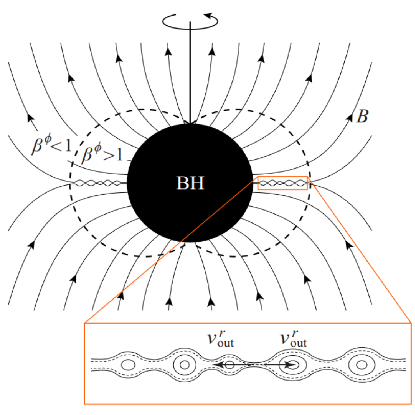
\includegraphics[width=0.5\textwidth]{figures/磁重联简介-8.pdf}
	\end{center}
	
	在初始条件的选择上，一般我们选取Fishbone和Moncrief于1976年提出的FMtorus模型，该模型给出了初始吸积盘的密度$\rho$、压强$p_g$、4-速$u^{\mu}$的分布。由于该模型是一个稳态模型，需要引入磁场使其不稳定（磁旋转不稳定性，MRI）而逐渐被黑洞吸积。为了使黑洞附近积累的磁力线足够多，一般我们选择初始磁场在整个吸积盘中都比较大：
	\begin{equation}
		A_{\phi} \propto (\rho - 0.01) (r \sin \theta / r_{\text{in}})^3 e^{- r / 400}
	\end{equation}
	其中$r_{\text{in}}$是吸积盘的内径。当磁力线被聚集到黑洞附近时，其位形类似于上图中的结构，因此磁重联大概率发生在赤道面附近。那么何时会发生磁重联呢？尽管磁重联随时可能发生，但我们倾向于认为其在磁通量爆发阶段更容易发生，也就是磁通量大幅度下降的时间段。这里的磁通量定义为：
	\begin{equation}
		\Phi_{\text{EH}} = \frac{1}{2} \int_{r = r_h} | B^r | \sqrt{\gamma} d \theta d \phi
	\end{equation}
	\begin{center}
		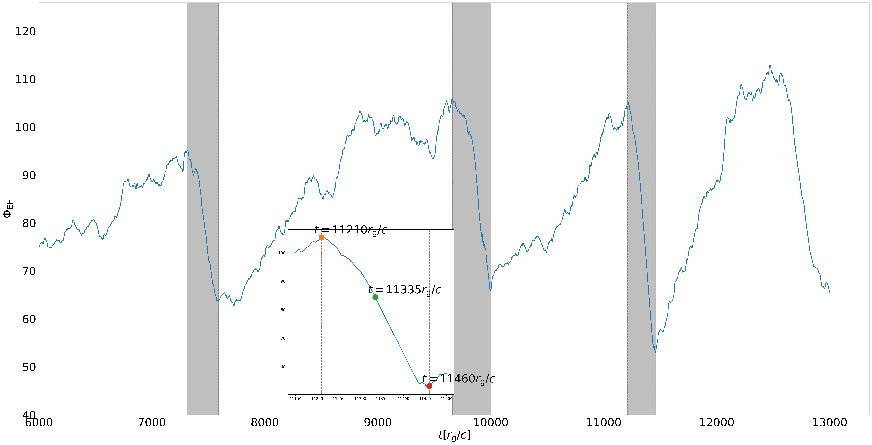
\includegraphics[width=0.9\textwidth]{figures/磁重联简介-9.pdf}
	\end{center}
	
	在确定了磁重联发生的时间和区域后，接下来最关键的就是找到磁重联事件了。然而，为了清晰地看到磁场精细结构，我们通常要求网格精度要求很高，这需要消耗巨大的计算资源。尽管如此，我们总是可以对这个时间段进行GRRT成像。
	
	\begin{center}
		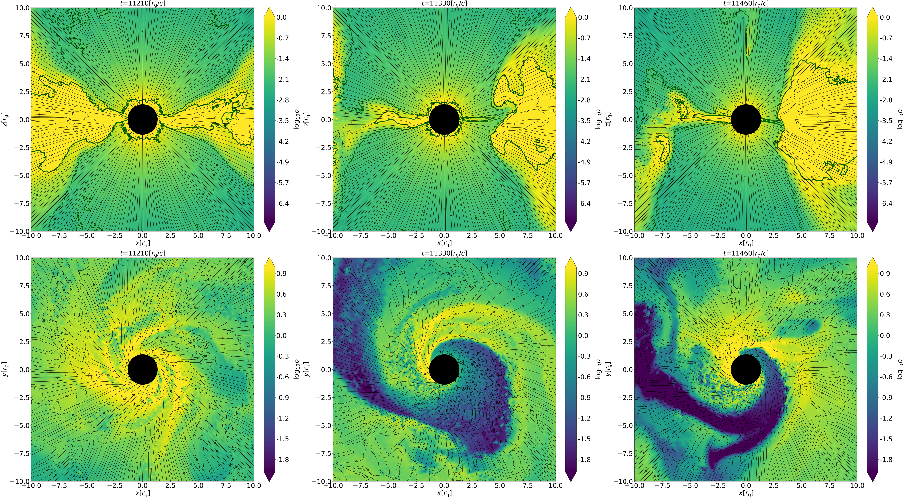
\includegraphics[width=\textwidth]{figures/磁重联简介-10.pdf}
	\end{center}
	
	\begin{center}
		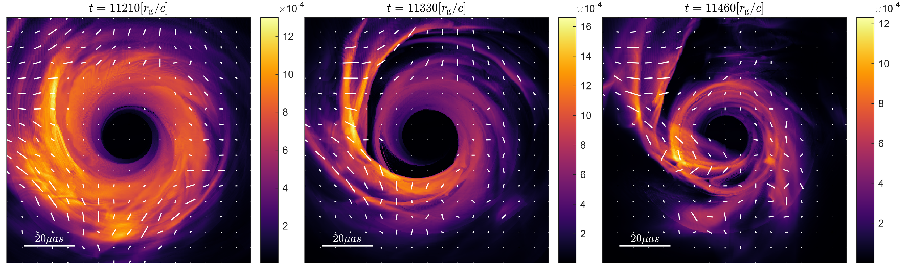
\includegraphics[width=\textwidth]{figures/磁重联简介-11.pdf}
	\end{center}
	
\nocite{*}
\printbibliography[heading=bibintoc,title=\ebibname]

\end{document}
